% start the document

% specify the document layout and font size
\documentclass[preprint,12pt]{elsarticle}
\usepackage[margin=1.5cm,includefoot]{geometry}
\usepackage{setspace}

% uploading packages
\usepackage{graphicx}
\usepackage{amssymb}
\usepackage{textcomp} % https://latex.org/forum/viewtopic.php?f=4&t=3364#p13124, https://tex.stackexchange.com/questions/165115
\usepackage{gensymb}
\usepackage{lineno}
\usepackage{mathtools}
\usepackage[separate-uncertainty=true]{siunitx}
\usepackage[colorlinks]{hyperref}
\usepackage[nameinlink,capitalise]{cleveref} %needs to appear after hyperref, https://tex.stackexchange.com/questions/396728/my-equations-referencing-not-working
\Crefname{figure}{Figure}{Figures} %needs to appear after hyperref and cleveref
\newcommand\crefrangeconjunction{--} % modify the reference style
\usepackage{mathrsfs}
\usepackage{url}
\usepackage{enumitem}
\usepackage{tabulary}
\usepackage{caption}
\usepackage{subcaption}
\usepackage{multirow}
\usepackage{makecell} % https://tex.stackexchange.com/questions/2441/how-to-add-a-forced-line-break-inside-a-table-cell
\newcommand{\NA}{---} % holds an m-dash
\graphicspath{{figures/}} %Setting the graphicspath
% ---------to deal with the double quotes----------- 
\usepackage [english]{babel}
\usepackage [autostyle, english = american]{csquotes}
\MakeOuterQuote{"}
%alternatively can use `` '' format for double quotes
\usepackage{booktabs}
\setlength{\abovetopsep}{1ex}
\usepackage[shortcuts,abbreviations]{glossaries-extra}
\newcommand*{\TCac}[1]{\ecapitalisewords{\glsentrylong{#1}}}

% figure info, etc. that can dynamically change (color of points, etc.)
\newcommand{\startpt}{red points}
\newcommand{\sympt}{dark blue points}
\newcommand{\refpt}{white circle}
\newcommand{\vbordercolor}{black}
\newcommand{\vcellcolor}{light blue}


\glssetcategoryattribute{abbreviation}{indexonlyfirst}{true}
\glssetcategoryattribute{abbreviation}{nohyper}{true}
\makeglossaries

\newabbreviation{5dof}{5DOF}{five degree-of-freedom}
\newabbreviation{ebsd}{EBSD}{electron backscatter diffraction}
\newabbreviation[longplural={grain boundaries}]{gb}{GB}{grain boundary}
\newabbreviation{fcc}{FCC}{face-centered cubic}
\newabbreviation{mfc}{MFC}{mass flow controller}
\newabbreviation{sem}{SEM}{scanning electron microscope}
\newabbreviation{fea}{FEA}{finite element analysis}
\newabbreviation{bcs}{BCs}{boundary conditions}
\newabbreviation[longplural={triple junctions}]{tj}{TJ}{triple junction}
\newabbreviation{gpr}{GPR}{Gaussian process regression}
\newabbreviation{ann}{ANN}{artificial neural network}
\newabbreviation{nn}{NN}{nearest neighbor}
\newabbreviation{rmse}{RMSE}{root mean square error}
\newabbreviation{mae}{MAE}{mean absolute error}
\newabbreviation{brk}{BRK}{Bulatov Reed Kumar}
\newabbreviation{gbed}{GBED}{grain boundary energy distribution}
\newabbreviation{gbcd}{GBCD}{grain boundary character distribution}
\newabbreviation{mfz}{MFZ}{misorientation fundamental zone}
\newabbreviation{bp}{BP}{boundary plane}
\newabbreviation{knn}{kNN}{k-nearest neighbor}
\newabbreviation{gbe}{GBE}{grain boundary energy}
\newabbreviation{gbo}{GBO}{grain boundary octonion}
\newabbreviation{oslerp}{oSLERP}{octonion Spherical Linear Interpolation}
\newabbreviation{loocv}{LOOCV}{leave-one-out cross validation}
\newabbreviation{kfcv}{kFCV}{k-fold cross validation}
\newabbreviation{seo}{SEO}{symmetrically equivalent octonion}
\newabbreviation{fex}{FEX}{file exchange}
\newabbreviation{idw}{IDW}{inverse-distance weighting}
\newabbreviation{fic}{FIC}{fully independent conditional}
\newabbreviation{svd}{SVD}{singular value decomposition}
\newabbreviation{gbc}{GBC}{grain boundary character}
\newabbreviation{fz}{FZ}{fundamental zone}
% \newabbreviation{pfz}{pFZ}{pseudo fundamental zone} % pfz replaced by vfz
% \newabbreviation{cmo}{CMO}{closed-mesh octonion} % cmo replaced by vfzo
\newabbreviation{vfz}{VFZ}{Voronoi Fundamental Zone}
\newabbreviation{vfzo}{VFZO}{Voronoi Fundamental Zone octonion}
\newabbreviation{lobpcg}{LOBPCG}{locally optimal block preconditioned conjugate gradient}
\newabbreviation{lkr}{LKR}{Laplacian kernel regression}
% example abbreviations
% \newabbreviation{seo}{SEO}{symmetrically equivalent octonions}
%\newabbreviation[longplural={grain boundaries}]{gb}{GB}{grain boundary}

%example usage: \gls{gpr}
%example usage: \Gls{gpr} (capitalize first letter, only meaningful for first usage)
% \glspl{seo} --> symmetrically equivalent octonions OR SEOs
%^^^^^^^^^^^^^^^^^^^^^^^^^^^^^^^^^^^^^^^^^^^^^^^^^^^


%\title{Grain Boundary Octonion Meshing and Interpolation}
\title{Five Degree-of-Freedom Property Interpolation of Arbitrary Grain Boundaries via \glsentrytitlecase{vfzo}{long} Framework}
\author[myu]{Sterling G. Baird}
\author[myu]{Eric R. Homer}
\author[myu]{David T. Fullwood}
\author[myu]{Oliver K. Johnson}\corref{cor1}

\address[myu]{Department of Mechanical Engineering, Brigham Young University, Provo, UT 84602, USA}
\cortext[cor1]{Corresponding author}
\date{October 2020}

% Double Spacing
% \doublespacing
\begin{document}

\begin{abstract}
    In this work we introduce the \gls{vfzo} interpolation framework for \gls{gb} structure-property models and surrogates. The \gls{vfzo} framework offers an advantage over other \gls{5dof} based property interpolation methods because it is constructed as a \gls{vfz} point set in a Riemannian manifold, for which Euclidean and arc length distances take on meaning and significantly reduce computation time compared with other distance metrics. This increased efficiency facilitates the use of significantly more input data and therefore leads to a reduction of the interpolation error. As a demonstration, we present \gls{gbe} interpolation results for a non-smooth validation function (Bulatov, Reed, Kumar) \cite{bulatovGrainBoundaryEnergy2014}.
    %and simulated bi-crystal datasets from the literature for Ni and Fe.
    Four interpolation methods built on this framework --- barycentric interpolation, \gls{gpr} or Kriging, \gls{idw}, and \gls{nn} interpolation --- are presented and compared against a constant, average model (\gls{rmse} $\simeq$ \SI{0.13}{\J\per\square\meter}), resulting in \gls{rmse} values of 0.063, 0.056, 0.068, and \SI{0.082}{\J\per\square\meter}, respectively, for \num{50000} randomly sampled input \glspl{gb} and evaluated for \num{10000} randomly sampled prediction \glspl{gb}. A vectorized, parallelized, MATLAB interpolation function is made available (\url{github.com/sgbaird-5dof/interp}). The \gls{vfzo} framework offers a great advantage in estimating property values for arbitrary \glspl{gb} and modeling surrogates of computationally expensive \gls{5dof} functions and simulations.
\end{abstract}

% 2020-10-24  The closed-octonion interpolation framework offers an advantage over other five-degree-of-freedom based property interpolation methods because it's defined as a closed mesh in a Riemannian manifold. One can triangulate a mesh using standard routines (e.g. quickhull, qhull.org) and interpolate using barycentric coordinates or machine learning methods such as Gaussian Process Regression. Euclidean and arc length distances take on meaning in this framework and are trivial computations compared with other distance metrics, thereby addressing a limitation in previous work. The ability to use significantly more input data lends itself to lower interpolation error and is demonstrated by grain boundary energy interpolation results for a non-smooth validation function (Bulatov, Reed, Kumar) and simulated bi-crystal datasets from the literature for Ni and Fe. Four interpolation methods built on this framework --- barycentric interpolation, Gaussian Process Regression or Kriging, inverse-distance weighting, nearest neighbor interpolation --- are presented and compared against a constant, average model (RMSE = 0.013 \J\per\square\meter), resulting in RMSE values of 0.063, 0.056, 0.068, and 0.082 \J\per\square\meter, respectively, for \num{50000} randomly input sampled bicrystals and evaluated for \num{10000} randomly sampled output bicrystals. A vectorized, parallelized, MATLAB implementation is made available (github.com/sgbaird-5dof/interp) with similar input/output structure of built-in MATLAB interpolation functions (e.g. \textit{interpn}) and placeholders for custom interpolation schemes. The closed-octonion framework offers a great advantage in estimating property values for arbitrary grain boundaries based on experimental or simulated data and modeling surrogates of computationally expensive 5DOF functions and simulations.

\maketitle

\section{Introduction} \label{sec:intro}

In this work, we present a new method for interpolation and prediction of grain boundary (GB) properties from a set of measured/calculated values. Our approach, called the \gls{vfzo} framework is highly efficient, and thereby facilitates the use of large data sets to enhance prediction accuracy.

\subsection{Previous Work}
In previous work, a number of strategies have been developed for describing a \gls{5dof} \gls{gb} property based on experimental or simulated data. Binning and gradient descent were used to produce a \gls{5dof} \gls{gbed} in nickel \cite{liRelativeGrainBoundary2009}, yttria \cite{dillonCharacterizationGrainboundaryCharacter2009}, and copper \cite{randleFiveparameterGrainBoundary2008} based on experimentally characterized 3D microstructures. 

A non-discretizing approach was recently introduced \cite{shenDeterminingGrainBoundary2019} that utilizes regularization imposed on \gls{tj} equilibrium equations, the \gls{lobpcg} method, and \gls{knn} distances. In this approach, \num{60000} \glspl{tj} (\num{180000} \glspl{gb}) and a custom, non-smooth validation function are used to obtain \gls{gbe} \gls{rmse} values of \SI{0.0076}{\J\per\square\meter} and \SI{0.0277}{\J\per\square\meter} for \gls{gbe} values greater than \SI{0.9}{\J\per\square\meter} and less than \SI{0.9}{\J\per\square\meter}, respectively. 

\citet{echeverrirestrepoUsingArtificialNeural2014} used an \gls{ann} and approximately \num{17000} and \num{51000} Fe bicrystal simulations from \citet{kimIdentificationSchemeGrain2011} as training and validation data, respectively, to achieve \glspl{mae} of \SI{0.0486}{\J\per\square\meter} and approximately \SI{0.09}{\J\per\square\meter} in the best fitted \glspl{ann} for randomly selected and special \glspl{gb}, respectively. 

Recently, a new \gls{gb} representation termed \glspl{gbo} was reported \cite{francisGeodesicOctonionMetric2019} and tested \cite{chesserLearningGrainBoundary2020}. The \gls{gbo} representation is valuable for a number of applications. Most relevant to the present work is the resulting distance metric. The \gls{gbo} distance metric offers an advantage over other metrics in that it "correctly determines the angular distances between \glspl{gb} with a common normal or misorientation" and "closely approximates the geodesic metric on $SO(3) \times SO(3)$ \textit{for all grain boundary pairs} while maintaining the ability to be analytically minimized with respect to the $U(1)$ symmetry" \cite{francisGeodesicOctonionMetric2019}. In this context, \citet{francisGeodesicOctonionMetric2019} derived \gls{oslerp} and provided examples showing that \gls{oslerp} produces smooth, minimum distance paths through \gls{gb} character space between two arbitrary \glspl{gb}. 

\Gls{lkr} (a type of \gls{idw}) involving scaled pairwise distance matrices was later used with \glspl{gbo} to predict properties of arbitrary \glspl{gb} from a set of known values \cite{chesserLearningGrainBoundary2020}. Using \gls{kfcv} with $k=10$ for \num{388} Ni \gls{gbe} simulations \cite{olmstedSurveyComputedGrain2009a} and an optimized scaling parameter, an \gls{rmse} of \SI{0.0977}{\J\per\square\meter} was obtained. Due to computation time of pairwise distance matrices, this approach is limited to datasets with several thousand \glspl{gb} or fewer \cite{chesserLearningGrainBoundary2020}.

\subsection{\glsentrytitlecase{vfzo}{long} Framework}
The \gls{vfzo} interpolation framework introduced in this work offers an advantage over other methods because it is defined as a \gls{vfz} point set in a Riemannian manifold. This is evidenced by the ability to triangulate a mesh using standard routines (e.g. quickhull \cite{barberQuickhullAlgorithmConvex1996}) and interpolate using barycentric coordinates or machine learning methods such as \gls{gpr}. Building on previous work on \glspl{gbo} \cite{francisGeodesicOctonionMetric2019,chesserLearningGrainBoundary2020}, we create a \gls{vfz} point set by obtaining a set of octonions minimized with respect to Euclidean distance and an arbitrary reference octonion after considering all \glspl{seo}. Because \glspl{gbo} are guaranteed to reside on the surface of a hypersphere \cite{francisGeodesicOctonionMetric2019} (a type of Riemannian manifold) a point set which locally resembles Euclidean space is formed (\cref{sec:methods:vfz-dist}). Below we mention a few benefits and applications of this approach, after which we provide the detailed description of the method (\cref{sec:methods}) and numerical test results (\cref{sec:results}).

\subsection{Benefits of \glsentrytitlecase{vfzo}{long} Framework}
\subsubsection{Distance Calculations}
Because Euclidean and arc length distances take on meaning in this framework, distance computations are much faster than other metrics. The calculation speed is even higher than explicit \gls{gbo} distance calculations using the original octonion distance given in \cite{francisGeodesicOctonionMetric2019}. For example, a \num{50000} x \num{50000} pairwise-distance matrix can be computed in approximately 70 s using built-in MATLAB \textit{Statistics and Machine Learning Toolbox} function \texttt{pdist} and 6 cores -- something that was computationally challenging before and a limitation of previous work. Compared to original octonion metric distance calculations \cite{chesserLearningGrainBoundary2020}, this represents an improvement in computational speed by five orders of magnitude!\footnote{Improvement per distance calculation per core is about \num{5e5} relative to the EMSoft \cite{degraefEMSoft2020} metric of 26 minutes using 8 cores for a 388 x 388 pairwise distance matrix in \cite{chesserLearningGrainBoundary2020}} This is largely due to the fact that \glspl{seo} only need to be considered once per \gls{gb} $L$, rather than once per distance calculation $L^2$,
%per \gls{gb} in a \gls{gb}-pair
and that \glspl{seo} only need to be considered once in a \gls{gb} pair $N_p^2$ rather than for every combination between the two \glspl{gb}\footnote{\texttt{GBdist.m} in \cite{chesserGBOctonionCode2019} uses the assumption that if a minimum angle is repeated 9 times, the symmetrization loop is exited, whereas the \texttt{GBmod.f90} implementation in EMSoft \cite{degraefEMSoft2020} does not appear to use this assumption.} ($N_p^4$). The computational complexity of this work is thus $O(N_p^2L)$, a significant improvement compared with the original complexity of $O(N_p^4L^2)$ \cite{chesserLearningGrainBoundary2020}, where $N_p$ is the symmetry cardinality ($N_p=24$ for $m\Bar{3}m$ \gls{fcc} point group) and $L$ is the number of \glspl{gb}. Additionally, Euclidean distances can be computed faster than trigonometric inverse functions, and built-in, vectorized MATLAB functions are utilized where possible. % $O(N^2L)$ (this work) vs. $O(N^4L^2$ (octonion paper)

\subsubsection{Interpolation Error} \label{sec:intro:interp-error}
The ability to use significantly more input data lends itself to lower interpolation error. This will be demonstrated by \gls{gbe} interpolation results for a non-smooth validation function in \cref{sec:results}.
%and simulated bi-crystal datasets from the literature (388 Olmsted Ni \cite{olmstedSurveyComputedGrain2009} and \num{50000} Kim Fe \cite{kimIdentificationSchemeGrain2011} bicrystals).
Four interpolation methods built on this framework --- barycentric (\cref{sec:methods:interp:bary}), \gls{gpr} or Kriging (\cref{sec:methods:interp:gpr}), \gls{idw} (\cref{sec:methods:interp:idw}), \gls{nn} (\cref{sec:methods:interp:nn}) --- will be presented and compared against a constant, average model (\cref{sec:results:accuracy}). To facilitate easy application of the presented method, a vectorized, parallelized, MATLAB implementation, \texttt{interp5DOF}, is made available \cite{bairdFiveDegreeofFreedom5DOF2020} with similar input/output structure to that of built-in MATLAB interpolation functions (e.g. \texttt{scatteredInterpolant(), griddatan()}) and placeholders for custom interpolation schemes. A typical function call is as follows: \texttt{ypred = interp5DOF(qm,nA,propList,qm2,nA2,method)}. Input misorientation quaternions (e.g. \texttt{qm}) and \gls{bp} normals (e.g. \texttt{nA}) define the input (\texttt{qm}, \texttt{nA}) and prediction or query points (\texttt{qm2}, \texttt{nA2}). Property values (\texttt{propList}) of \glspl{gb} corresponding to the (\texttt{qm},\texttt{nA}) pairs are supplied. Internally, these are converted to octonions and interpolated or predicted values (\texttt{ypred}) corresponding to the \texttt{qm2}/\texttt{nA2} pairs are returned based on the selected \texttt{method}. The methods used in this work are \texttt{'pbary'}, \texttt{'gpr'}, \texttt{'idw'}, and \texttt{'nn'}, corresponding to planar barycentric, \gls{gpr}, \gls{idw}, and \gls{nn} interpolation, respectively, and a placeholder template with instructions is provided in \texttt{interp5DOF}. Misorientation quaternions are represented in the active sense\footnote{The passive convention is used in \cite{francisGeodesicOctonionMetric2019}}:
\begin{equation}
    q_m = {q_A}^{-1}q_B
\end{equation}
where $q_m$, $q_A$, and $q_B$ represent the misorientation quaternion, quaternion of grain A in the sample frame, and quaternion of grain B in the sample frame, respectively. The $^{-1}$ operator denotes a quaternion inverse. \Gls{bp} unit normals are expressed pointing away from grain A and in the reference frame of grain A (i.e. the outward-pointing normal convention). See \cite{francisGeodesicOctonionMetric2019} for a treatment of conversions to octonion coordinates.

\subsubsection{Applications}

The \gls{vfzo} framework offers a great advantage in estimating property values for arbitrary \glspl{gb} based on experimental or simulated data such as energy, mobility, and diffusivity. The framework can also enable efficient surrogate modeling of computationally expensive 5DOF functions and simulations such as in evaluation of the \gls{brk} function for use in anisotropic grain growth simulations. In other words, one can evaluate the \gls{vfz} surrogate model in a fraction of the time of the true property model, thereby facilitating larger scale iterative simulations, which require repetitive evaluation of a computationally expensive structure-property model.

% We think it is straightforward to apply these methods to full or restricted regions of \gls{5dof} space for \gls{gb} models and surrogates. In addition to interpolations involving \gls{gbe}, \gls{gbcd} (i.e. similar to fitting a curve to a histogram) and other \gls{gb} properties such as diffusivity and mobility could also be interpolated. Finally, linking this interpolation scheme with polycrystal data such as 3D microstructural \gls{tj} datasets (e.g. Ni \cite{liRelativeGrainBoundary2009}) via \textit{TJ2GBE} \cite{shenDeterminingGrainBoundary2019} or similar approaches geared towards large datasets is especially promising.

\section{Methods} \label{sec:methods}

The core operations of the \gls{vfzo} framework are (i) the generation of, and (ii) mapping of points into, a \gls{vfz}, and (iii) distance calculations within the \gls{vfz}. Rather than relying on an analytically defined \gls{fz}, we employ a numerical approximation, which we will refer to as a \gls{vfz}.

The construction of the \gls{vfz} dramatically reduces the computational burden of pairwise distance calculations. The mechanism by which this reduction is achieved can best be illustrated with an example. Let $o_1$ and $o_2$ denote two \glspl{gb} represented as octonions, or \glspl{gbo}. 
To perform a traditional distance calculation it is necessary to compare all \glspl{seo} of $o_1$ to all of the \glspl{seo} of $o_2$ and take the smallest distance. If $N_p$ is the cardinality of the crystallographic point group, this single minimum distance calculation requires a total of $N_p^4$ \glspl{seo} to be considered. If one desires to compute a pairwise distance matrix between $L$ GBs, the total number of \glspl{seo} computations will be $O(N_p^4L^2)$.

In contrast, for a single distance calculation using the \gls{vfzo} framework, $o_1$ and $o_2$ are first mapped into the \gls{vfz}, and then only a single distance calculation is required between them. Mapping $o_1$ into the \gls{vfz} requires comparison of all $N_p^2$ \glspl{seo} of $o_1$ with a fixed reference \gls{gb} in the interior of the \gls{vfz}; and likewise for $o_2$. Consequently, a single distance calculation between $o_1$ and $o_2$ under the \gls{vfzo} framework requires $2N_p^2$ \gls{seo} computations. If one desires to compute a pairwise distance matrix between $L$ \glspl{gb}, the total computational cost will be $O(N_p^2L)$, which represents a dramatic reduction. A summary of the differences between the two approaches is provided in \cref{tab:closed-mesh-comparison}.

\begin{table}
\caption{Comparison between \acrlong{vfzo} and traditional octonion frameworks. *6D Cartesian representation used only for mesh triangulation efficiency in barycentric interpolation and *7D Cartesian representation only required for barycentric interpolation. For pairwise distance complexity, $N_p$ is the symmetry cardinality ($N_p=24$ for $m\Bar{3}m$ \gls{fcc} point group) and $L$ is the number of \glspl{gb}.}
\centering
\begin{tabular}{ccc}
\toprule
Property & Traditional & This Work \\
\midrule
Symmetrizing Distance & Octonion & Euclidean \\
Considered \glspl{seo} & Subset & All \\
Dimensionality & 8D Cartesian & 6*/7*/8D Cartesian \\
Riemannian Mesh & No & Yes \\
% Euclidean Approximation Valid & No & Yes \\
Pairwise Distance Complexity & $O(N_p^4L^2)$ & $O(N_p^2L)$ \\
\bottomrule
\end{tabular}
\label{tab:closed-mesh-comparison}
\end{table}

In this section we describe our methods for each of the \gls{vfzo} framework operations (i)-(iii) named above. We then describe our implementation of 4 different interpolation schemes for prediction of \gls{gb} properties based on the \gls{vfzo} approach.

\subsection{The \glsentrytitlecase{vfzo}{long} Framework}
\label{sec:methods:framework}

\subsubsection{Defining the \glsentrytitlecase{vfz}{long}}
\label{sec:methods:vfz}

% Explain the "voronoi" type definition of the vfz by choosing a reference GB and then taking the symmetric image of each GB that is closest to that reference GB. You will need to convince the reader (probably by reason, or proof, or numerical tests) that the resulting vfz does in fact contain one and ONLY one SEO for every GB (i.e. that it does satisfy the definition of a FZ). This is probably where you note that for it to work, the reference GB needs to be something that isn't a high-symmetry GB, and why. This discussion will probably benefit from a figure illustrating the procedure in 2D.

In order to define a \gls{vfz}, an arbitrary, fixed, low-symmetry reference \gls{gbo} is chosen ($o_{ref}$) which will define the \gls{vfz}. To illustrate, we describe a 3D Cartesian analogue (\cref{fig:voronoi}) to a 7D Cartesian representation of a \gls{vfz}. A set of \num{500} points ($p_i, i\in[1,500]$) randomly scattered on the surface of the 2-sphere comprise the data (\startpt) and a random point, also on the surface of the 2-sphere, defines the reference point, $p_{ref}$ (\refpt). In this analogy, $O_h$ or $m\bar{3}m$ point group rotations are used as symmetry operators, $S_j,j\in[1,N_p]$, where $N_p$ is the cardinality as before and $N_p = 24$ for the $O_h$  point group. For each data point, \num{24} symmetrically equivalent representations ($p^{sym}_{i,k},k\in[1,24]$) are produced by applying the appropriate rotation transformations ($S_j(p_i),j\in[1,24]$). After calculating the Euclidean distance between $p_{ref}$ and $p^{sym}_{i,k},k\in[1,24]$, the point closest to $p_{ref}$ is chosen ($p^{NN}_i,i\in[1,500]$) and retained in a newly defined \gls{vfz}.

The minimum Euclidean distance \gls{seo} will be the same as the minimum arc length distance \gls{seo} because arc length ($s(x)$) is a monotonically increasing function of Euclidean distance ($x$) in $s(x)\in[0,\pi]$ (\cref{fig:dist-parity}). Without loss of generality, $s(2)=\pi$ gives the maximum arc length that can be obtained from two points on a unit-sphere and $2$ is the maximum Euclidean distance (diameter of a unit-sphere).

This approach can also be described in the context of a Voronoi tessellation. In the 3D Cartesian example (\cref{fig:voronoi}), all symmetrically equivalent representations of $p_{ref}$ are used to define a Voronoi tessellation on the 2-sphere, portrayed as \vcellcolor cells with \vbordercolor borders. The symmetrized points ($p^{NN}_i,i\in[1,500]$) (\sympt) described previously uniquely fall within a single Voronoi tessellation cell of $p_{ref}$, resulting in a \textit{\gls{vfz} point set}.

\begin{figure}
    \centering
    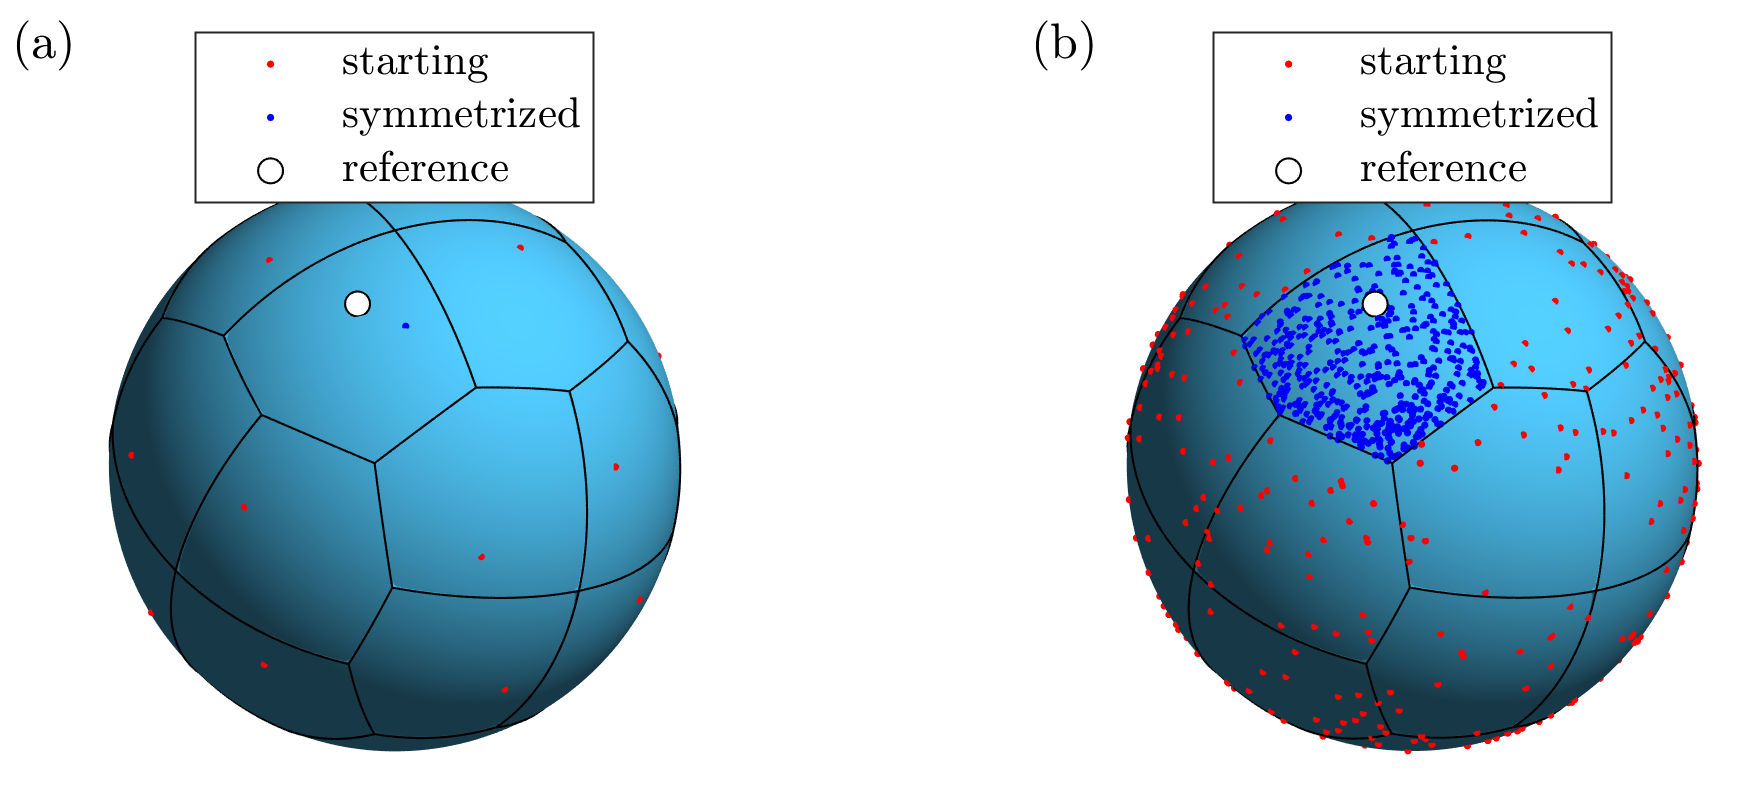
\includegraphics[scale=1]{voronoi.png}
    \caption{3D Cartesian analogue to a 7D Cartesian representation of \glspl{gbo} and \glspl{vfzo} demonstrating a single input point (\startpt) that is symmetrized (\sympt) relative to a fixed, reference point (\refpt) (a). Only one symmetrized point is found within the borders (\vbordercolor) of each of the Voronoi cells (\vcellcolor), where the Voronoi tessellation is defined by the symmetric images of the reference point. (b) shows demonstrates the symmetrization of many points, leading to a 3D Cartesian \gls{vfz} point set.}
    \label{fig:voronoi}
\end{figure}

The expectation that a single, unique \gls{seo} will be found (within numerical tolerance and given a low-symmetry reference \gls{gbo}) is verified by several manual tests and internally within the symmetrization function \texttt{get\_octpairs()} \cite{bairdFiveDegreeofFreedom5DOF2020}. Similar manual tests reveal that a high-symmetry reference \glspl{gbo} results in many degenerate minimum distance \glspl{seo}, with the identity octonion ($\{1,0,0,0,0,0,0,0\}\in\mathbb{R}^8$) \cite{francisGeodesicOctonionMetric2019} giving the highest degeneracy.

\subsubsection{Mapping \glsfmtshortpl{gb} to the \glsentrytitlecase{vfz}{long}}
\label{sec:methods:proj}

% With the reference GB chosen, and consequently the vfz defined, explain that a GB is mapped into the vfz simply by finding among its \glspl{seo} the one that is closest to the reference GB.

With a reference \gls{gbo} chosen ($o_{ref}$), and consequently the \gls{vfz} defined (\cref{sec:methods:vfz}), a \gls{gb} is mapped into the \gls{vfz} by finding among its \glspl{seo} the one that is closest to $o_{ref}$. This is performed for all input and prediction points w.r.t. $o_{ref}$ resulting in a \gls{vfz} point set.

% In the \gls{vfzo} framework, \glspl{seo} are chosen based on minimum Euclidean distance relative to a fixed, arbitrary reference octonion rather than allowing either octonion in a pair to vary in the traditional octonion approach with arc-length distances \cite{francisGeodesicOctonionMetric2019}. We consider all symmetrically equivalent \glspl{gbo} rather than a subset. For barycentric interpolation (\cref{sec:methods:bary}), we also remove a degenerate dimension via a rigid \gls{svd} transformation to 7D Cartesian and employ a further projection to 6D Cartesian only for the triangulation. These differences are summarized in Table \cref{tab:closed-mesh-comparison}. By choosing \glspl{seo} based on Euclidean distance with respect to a fixed octonion, a "closed-mesh" is obtained in the sense that directly computed Euclidean and arc length distances become meaningful and a unique octonion is found within numerical tolerance as long as the reference \gls{gbo} is low-symmetry (very likely based on random sampling and can be verified). This facilitates the use of standard triangulation and interpolation routines rather than needing to rely on pairwise-distance matrices where each distance calculation requires consideration of \glspl{seo}.

\subsubsection{Generating Random \glsentrytitlecase{vfzo}{long}}
\label{sec:methods:rand}
First, random \glspl{gbo} are formed by taking a random, cubochorically sampled quaternion \cite{singhOrientationSamplingDictionarybased2016} \texttt{qm} and random \gls{bp} unit vector \texttt{nA} pair and converting these to an octonion representation \texttt{o} using a modified version \cite{bairdFiveDegreeofFreedom5DOF2020} of \texttt{GBfive2oct()} \cite{chesserGBOctonionCode2019} via \texttt{o=GBfive2oct(qm,nA)}. The conventions used for \texttt{qm} and \texttt{nA} are given in \cref{sec:intro:interp-error}. After mapping random \glspl{gbo} (\cref{sec:methods:rand}) into the \gls{vfz} (\cref{sec:methods:proj}) to obtain \glspl{vfzo} % ...

\subsubsection{Distance Calculations in the \glsentrytitlecase{vfz}{long}}
\label{sec:methods:vfz-dist}

% Explain how to compute distances in the vfz, and why you can now just use euclidean distances.
The \gls{vfz} is defined such that directly computed Euclidean and arc length distances are meaningful. Euclidean distances are an accurate approximation of arc length distances in a \gls{vfz} because the difference between the two metrics for the maximum pairwise distance ($pd_{max} = \SI{60}{\degree})$) in a \gls{vfz} is small as shown in \cref{fig:dist-parity}. However, due to the presence of low-symmetry \glspl{gb} near the exterior of a \gls{vfz}, some \glspl{gb} pairs will exhibit larger distances than is truly representative (\cref{fig:dist-ensemble-k1-2-5-10}). In other words, moving "past" the low-symmetry border of a \gls{vfz} will result in an instantaneous relocation to a possibly distant point in the \gls{vfz} that in reality is highly correlated.

\begin{figure}
\centering
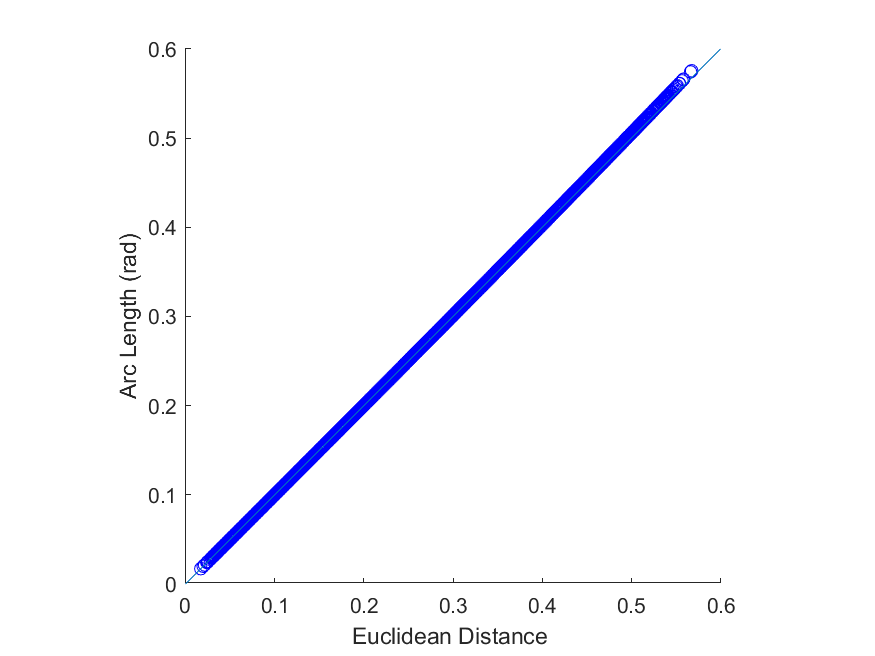
\includegraphics[scale=1]{dist-parity.png}
\caption{Parity plot of hyperspherical arc length vs. Euclidean distance for pairwise distances in a symmetrized, \gls{vfz} point set of \num{10000} randomly sampled \acrlongpl{gbo}. The max arc length is approximately \SI{0.58}{\radian}, indicating a max octonion distance of approximately \SI{1.16}{\radian} or \SI{66.5}{\degree} between any two points in the \acrlong{fz}. The close correlation between arc length and Euclidean distance supports the validity of using Euclidean distance in the interpolation methods.}
\label{fig:dist-parity}
\end{figure}

This is a limitation of the \gls{vfzo} framework which generates a \gls{vfz} with low-symmetry \glspl{gb} at the borders in contrast to typical \glspl{fz} \cite{patalaSymmetriesRepresentationGrain2013,homerGrainBoundaryPlane2015}. While defining a \gls{fz} with high-symmetry \glspl{gb} at the borders will certainly increase interpolation accuracy, the favorable interpolation results presented in this work are obtained because overestimation is infrequent within a small correlation length (e.g. \SI{10}{\degree}).

Overestimation imposes an arbitrary "sparseness" of data within a local region of influence common to the interpolation methods in this work, whereas underestimation would give erroneous high correlations between uncorrelated \glspl{gb}. Because only overestimation relative to traditional octonion distances exist in this work (\cref{fig:dist-ensemble-k1-2-5-10}), it is expected that large errors will occur infrequently, as shown in \cref{fig:brkparity50000}, and that overall errors will remain low as shown in \cref{fig:brkerror}, \cref{tab:rmse-error-comparison}, and \cref{tab:mae-error-comparison}. We find that taking the minimum distance among several \gls{vfzo} sets defined by separate reference octonions leads to better correlation between the Euclidean approximation and the traditional octonion metric (\cref{fig:dist-ensemble-k1-2-5-10} and \cref{fig:dist-ensemble-rmse-mae}). We plan to explore the incorporation of ensemble \gls{vfzo} sets to interpolation methods and expect increased accuracy at reasonable computational cost.

Certain simplex-based approaches \cite{connorHighdimensionalSimplexesSupermetric2017,boissonnatOnlyDistancesAre2017} may allow for other \gls{gb} distance metrics \cite{morawiecDistancesGrainInterfaces2019} to be paired with the triangulation facets computed in the barycentric interpolation approach (\cref{sec:methods:interp:bary}) and is a topic of interest for future study.

% Because a fixed, arbitrary, reference octonion is used to symmetrize the mesh, meshes with different exterior bounds can be obtained based on the reference octonion used. This is a limitation of this work in that the boundaries of the mesh do not correspond with high-symmetry \glspl{gb} in contrast with typical \gls{fz} representations in misorientation or \gls{bp} \cite{patalaSymmetriesRepresentationGrain2013,homerGrainBoundaryPlane2015} spaces. Interpolated values near the exterior of the mesh are likely to have higher error because the local region of influence may be prematurely cut off for \gls{gpr} and \gls{idw}. By definition of the barycentric and \gls{nn} methods, extrapolation is necessary to predict values on or near the "true" boundary of the mesh due to expected curvature in those boundaries. Further, \gls{nn} and barycentric interpolation are the only two non-smooth interpolation methods used; in these two cases, sharp cusps in the model will be smoothed or misrepresented unless there are \glspl{gb} on the cusp. For \gls{gpr} and \gls{idw}, cusps will be smoothed by definition as long as there is a non-zero kernel and non-zero standard deviation employed. This is a feature common to previously published methods \cite{liRelativeGrainBoundary2009,shenDeterminingGrainBoundary2019,chesserLearningGrainBoundary2020} except for those \cite{bulatovGrainBoundaryEnergy2014,shekhawatGeneralizedReadShockley2016} which explicitly implement the Read-Shockley model \cite{readDislocationModelsCrystal1950}. For a discussion of possible ways to address these issues, see Section \cref{sec:conclusions:future}.

\begin{figure}
    \centering
    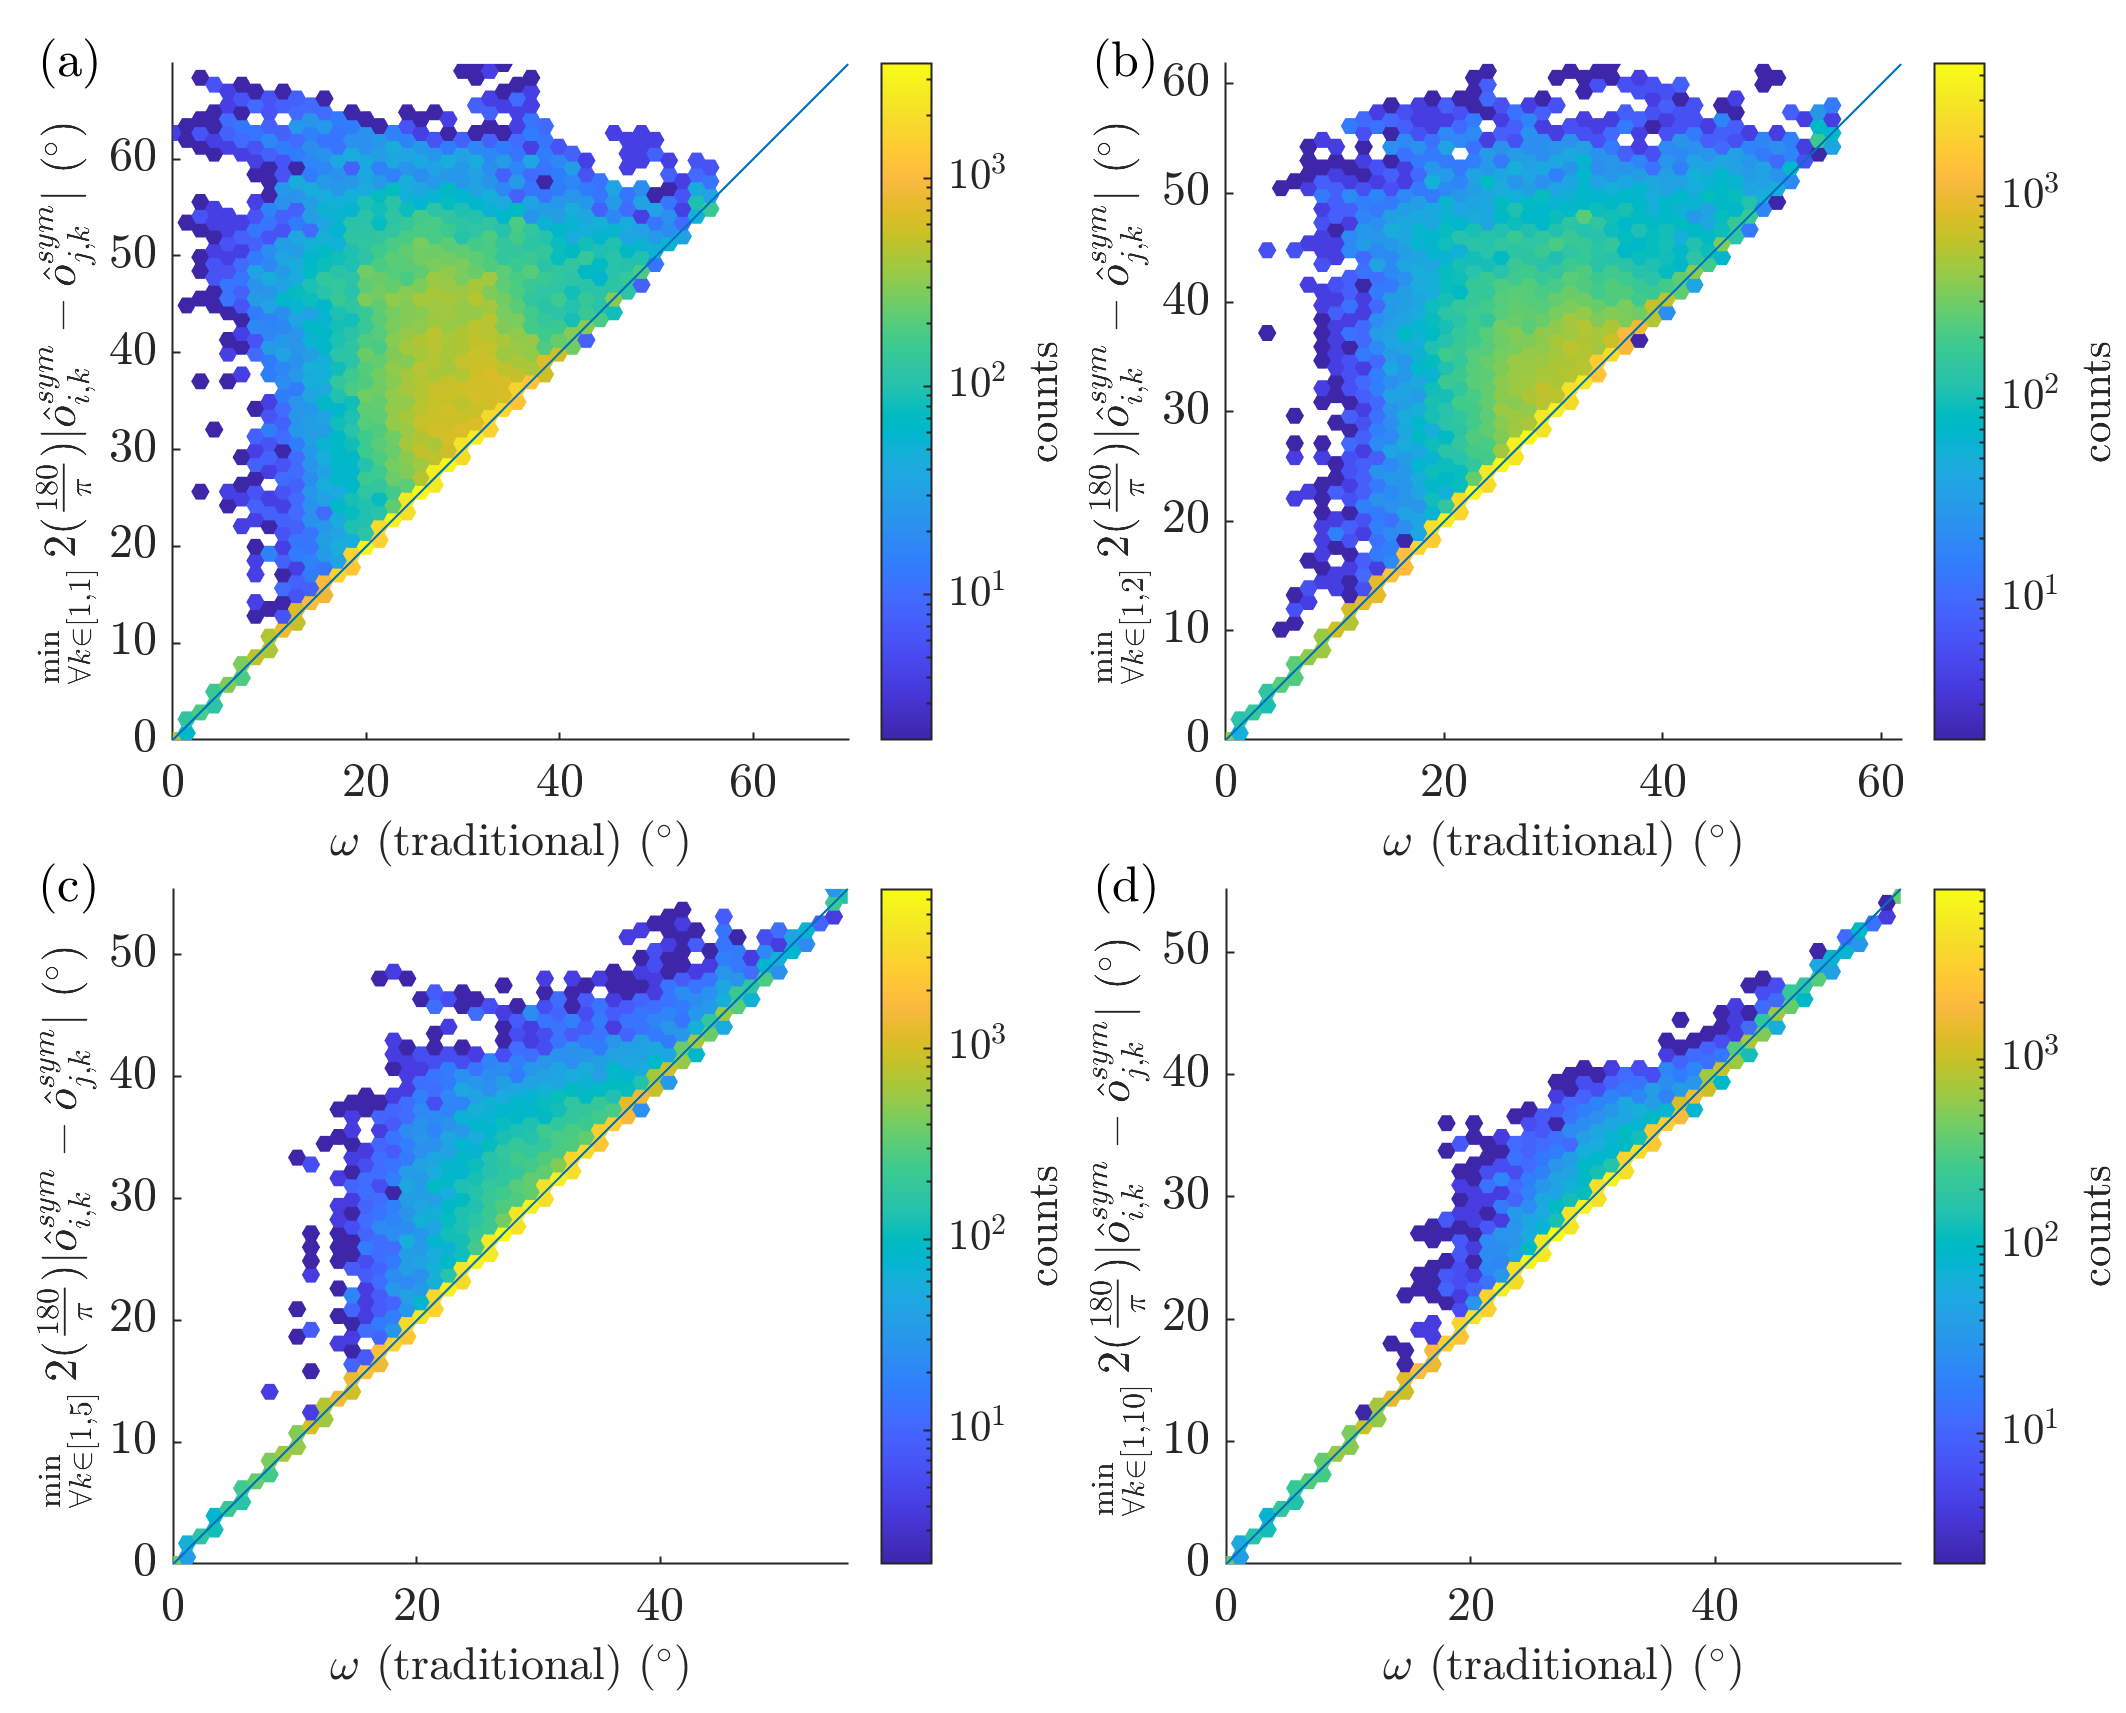
\includegraphics[scale=1]{figures/dist-ensemble-k1-2-5-10.png}
    \caption{Hexagonally binned parity plots of pairwise distances of 388 Ni bicrystals \cite{olmstedSurveyComputedGrain2009a}. Euclidean distance approximation is converted to octonions ($x_{i,j,k}=2\frac{180}{\pi}|\hat{o}_{i,k}^{sym}-\hat{o}_{j,k}^{sym}|$) for comparison with the traditional octonion metric \cite{chesserLearningGrainBoundary2020}. The minimum distance among an ensemble of \gls{vfzo} sets ($\min_{\forall k \in [1,k_{max}]}x_{i,j,k}$) is used for 1 (a), 2 (b), 5 (c), and 10 (d) \gls{vfzo} sets. As the number of \gls{vfzo} sets increases, the correlation between the Euclidean distance and the traditional octonion distance improves.}
    \label{fig:dist-ensemble-k1-2-5-10}
\end{figure}

\subsection{Interpolation in the \glsentrytitlecase{vfzo}{long} Framework}
\label{sec:methods:interp}

\subsubsection{Barycentric Interpolation}
\label{sec:methods:interp:bary}

% Give brief explanation of standard barycentric interpolation: you find which simplex the point is in, then you calculate the weights. The advantage of this approach is that the weight matrix only has to be computed once. If you interpolate different functions over the same query points, the weights don't change, so re-evaluation with a new function is rapid via a simple matrix multiplication.

% Explain how to adapt barycentric interpolation to the vfz: how to identify which simplex the query point falls in, and then how to compute the weights. Also explain and justify why you can use euclidean distances (i.e. because the vfz occupies a small portion of the 7-sphere it is nearly planar so euclidean distances and octonion distances are approximately equal and you can show tha figure here), and how that speeds things up.

Barycentric coordinates are a type of homogeneous coordinate system that reference a prediction point within a simplex \cite{langerSphericalBarycentricCoordinates2006} or convex polytope \cite{floaterGeneralizedBarycentricCoordinates2015,meyerGeneralizedBarycentricCoordinates2002,langerSphericalBarycentricCoordinates2006} based on "masses" or weights at the vertices. The prediction point is assumed to be the barycenter (center of mass) of the simplex or convex polytope, and weights at the vertices necessary to make this assumption true are determined. We utilize rigid \gls{svd} transformations and a standard triangulation algorithm to define a simplicial mesh (\cref{app:bary-tri}). We then use barycentric weights (i.e. coordinates) for computing intersections of a point within a simplicial facet (\cref{app:bary-int}) and for interpolation (\cref{app:bary-interp}) \cite{langerSphericalBarycentricCoordinates2006}.

\subsubsection{\glsentrytitlecase{gpr}{long}}
\label{sec:methods:interp:gpr}

% You don't need to give a detailed explanation of GPR, but you do need 1 sentence summarizing the idea and then point to REF for a general treatment. Explain any assumptions or adaptations that need to be done to use it with the vfz (e.g. presumably GPR is not actually operating on the surface of the 7-sphere, rather it is actually operating on all of $\mathbb{R}^8$, but because the vfz occupies a small portion of the 7-sphere it is nearly planar so euclidean distances and octonion distances are approximately equal, as mentioned previously, so it works without modification). Finally just explain that we used matlab's built-in \texttt{fitrgp()} function and the options used like you already have written.

\Gls{gpr} or kriging uses the notion of similarity between points to fit Gaussian processes (random variables) to data based on prior information and provides uncertainty information in addition to interpolated or inferred values. For a general treatment of \gls{gpr}, see \cite{rasmussenGaussianProcessesMachine2006}. We use MATLAB's built-in function, \texttt{fitrgp}, with all default parameters (MATLAB R2020b) except that \texttt{PredictMethod = 'exact'} regardless of the number of input points, and we assume a Euclidean approximation of the \gls{vfz} (\cref{sec:methods:vfz-dist}, \cref{fig:dist-parity}). A faster, less memory-intensive \gls{fic} approximation is also available (\texttt{PredictMethod = 'fic'}).

\subsubsection{\glsentrytitlecase{idw}{long} Interpolation}
\label{sec:methods:interp:idw}

% Explain the idea behind IDW in 1 sentence, then give the details of how you implemented it and any adaptations that are necessary for the present situation.

\Gls{idw} applies a weighted average to points within a neighborhood of a query point to obtain an interpolated value. A simple \gls{idw} approach is implemented based on a MATLAB \gls{fex} submission \cite{tovarInverseDistanceWeight2020}. A default radius of influence of $r=\sqrt{2} \mu$ is used, where $\mu$ represents mean \gls{nn} distance, and where octonion distance is approximated by the Euclidean distance or 2-norm (\cref{sec:methods:vfz-dist}, \cref{fig:dist-parity}). \gls{nn} (\cref{sec:methods:interp:nn}) is used for a given query point when there are no points in the radius of influence.

\subsubsection{\glsentrytitlecase{nn}{long} Interpolation}
\label{sec:methods:interp:nn}

% Again, explain the idea in 1 sentence, and then give any special adaptations necessary.

\Gls{nn} takes the nearest input point relative to a query point and assigns the value of the \gls{nn} input point to the query point. This is implemented via the built-in MATLAB function \texttt{dsearchn} using a Euclidean approximation of octonion distance (\cref{sec:methods:vfz-dist}, \cref{fig:dist-parity}).

% ---the rest of the methods section is what you previously wrote, I'm leaving it here so that you can use pieces of it for the v2.0 framework I implemented above, but once you've copied the portions you need go ahead and delete the remainder of the methods section below here---
%----------------------------old draft-----------------------
% \subsection{\glsentrytitlecase{vfzo}{long} vs. Traditional Octonion Frameworks} \label{sec:methods:closed-mesh-comparison}

% \subsubsection{Defining a Closed-mesh}
% In the \gls{vfzo} framework, \glspl{seo} are chosen based on minimum Euclidean distance relative to a fixed, arbitrary reference octonion rather than allowing either octonion in a pair to vary in the traditional octonion approach with arc-length distances \cite{francisGeodesicOctonionMetric2019}. We consider all symmetrically equivalent \glspl{gbo} rather than a subset. For barycentric interpolation (\cref{sec:methods:bary}), we also remove a degenerate dimension via a rigid \gls{svd} transformation to 7D Cartesian and employ a further projection to 6D Cartesian only for the triangulation. These differences are summarized in Table \cref{tab:closed-mesh-comparison}. By choosing \glspl{seo} based on Euclidean distance with respect to a fixed octonion, a "closed-mesh" is obtained in the sense that directly computed Euclidean and arc length distances become meaningful and a unique octonion is found within numerical tolerance as long as the reference \gls{gbo} is low-symmetry (very likely based on random sampling and can be verified). This facilitates the use of standard triangulation and interpolation routines rather than needing to rely on pairwise-distance matrices where each distance calculation requires consideration of \glspl{seo}.



% Separate from the mesh \textit{triangulation}, mesh \textit{intersections} are calculated via a new transformation of the original 8D Cartesian octonions to 7D Cartesian coordinates that includes a simultaneous transformation of two sets -- input points and prediction points -- to preserve distances and angles \textit{between each set} as well as \textit{within each set}. Despite having different \glspl{svd}, the 6D Cartesian triangulation holds for either 7D Cartesian representation (triangulation or intersection) because the two 7D Cartesian representations are rigid to each other (i.e. distance- and angle-preserving). However, for prediction points to have meaning with respect to the input point mesh, the intersections between these two must be calculated using a \gls{svd} involving both simultaneously as described here.
%There are approximately 1900 facets per point, 7 vertices per facet, and \num{1e8} total facets for a \num{50000} point mesh in 7D Cartesian.
    
% \subsection{Gaussian Process Regression or Kriging} \label{sec:methods:gpr}

% The implemented \gls{gpr} scheme uses MATLAB's built-in function, \texttt{fitrgp} with default parameters in MATLAB R2020b except for \texttt{PredictMethod}, which is set to \texttt{'exact'} regardless of the number of input points. For a general treatment of \gls{gpr}, see \cite{rasmussenGaussianProcessesMachine2006}. A number of non-default settings -- \texttt{FitMethod}, \texttt{PredictMethod}, \texttt{OptimizeHyperarameters}, and \texttt{ActiveSetMethod} -- were tested and resulted in marginal error improvement relative to results produced by the default parameters which usually also resulted in a deficit in time performance; however, custom \texttt{fitrgp} options can still be passed into \texttt{interp5DOF} \cite{bairdFiveDegreeofFreedom5DOF2020}. For faster, less accurate, and less memory-intensive computations consider using \gls{fic} (\texttt{'fic'}) approximation as the \texttt{PredictMethod} instead. % as summarized in the table below.

% \item MATLAB fitrgp
%         \begin{enumerate}
%             \item squared exponential covariance function
%             \item bcd fit method (others are sd, fic etc.)
%             \item constant basis function
%             \item exact or bcd predict methods (also fic)
%             \item quasi-newton optimizer
%             \item optimize KernelScale and Sigma hyperparameters with bayesopt Optimizer
%             \item ActiveSetMethod - entropy (others, log likelihood, sparse greedy approximation)
%         \end{enumerate}

% \subsection{Inverse-Distance Weighting} \label{sec:methods:idw}

% A simple \gls{idw} approach is implemented similar to a MATLAB \gls{fex} submission \cite{tovarInverseDistanceWeight2020}. A pairwise distance matrix is computed and distances outside of a specified radius $r$ are ignored, and $r$ given by a scaled version of the mean of the \gls{nn} pairwise Euclidean distance matrix: 
% \begin{equation}
% r=\sqrt{2} \mu
% % r=\frac{\mu }{\sqrt{2}}
% % r=\frac{\sum _{k=1}^N \sum _{j=1}^N \sqrt{\sum _{i=1}^N \left(x_{i,j}-x_{i,k}\right){}^2}}{\sqrt{2} N},j\neq k
% % where $r$, $x_{i,j}$, $x_{i,k}$, and $N$ represent the radius of influence, $i$th component of the $j$th point, $i$th component of the $k$th point, and total number of points, respectively.
% \end{equation}
% where $r$ and $\mu$ represent the radius of influence and mean \gls{nn} distance, respectively. Euclidean distance is used by default to define the weight matrix via $W_{i,j} = \frac{1}{D_{i,j}^L}$, where $i,j$ gives the $i$th row and $j$th column and $W$, $D$, and $L$ represent the weight matrix, pairwise-distance matrix, and norm-power (i.e. $L = 2$ for Euclidean), respectively. For prediction points that have no input mesh points within the specified radius, the \gls{nn} approach is used instead (\cref{sec:methods:nn}). The rest of the interpolated prediction point values are computed normally using \gls{idw} as described.

% \subsection{Nearest Neighbor} \label{sec:methods:nn}

% \Gls{nn} is one of the simplest interpolation schemes implemented using the built-in MATLAB function \texttt{dsearchn}. Euclidean distance will produce the same results as octonion distance for this method. \Gls{nn} computations are fast due to the simple calculation of Euclidean distance and ability to use optimized, built-in methods.

% \subsection{Random Grain Boundary Sampling} \label{sec:methods:rand}

% Random sampling of \glspl{gb} occurs in \gls{5dof} space by taking a random, cubochorically sampled quaternion and random unit vector \gls{bp} normal as a pair and then converting from this \gls{5dof} representation to a \gls{gbo}. All random sampling of octonions reported in this work take place via this scheme.

% % \begin{enumerate}
    
%     % \item Gaussian process regression
%     % \begin{enumerate}
        
%     % \end{enumerate}
    
% % \end{enumerate}

\section{Results and Discussion} \label{sec:results}

To illustrate the utility of the \gls{vfzo} framework for one application, namely interpolation, we compare the (i) accuracy, and (ii) efficiency of the four previously described interpolation methods implemented over the \gls{vfz} with each other and with existing methods from the literature (see \cref{sec:intro}).

For these tests, we used the 5DOF GB energy function developed by Bulatov, Reed and Kumar \cite{bulatovGrainBoundaryEnergy2014}, as the test function. First a \gls{vfz} point set is randomly generated, corresponding to an average mesh resolution and standard deviation of about \SI{2.87}{\degree} and \SI{0.7}{\degree}, respectively (\cref{fig:nnhist-knn-50000}). We denote this set of \glspl{gb} by \texttt{gb\_v}. The test function was then evaluated at each of these points and the values were stored in the vector \texttt{f\_v}. We then generated \num{10000} query \glspl{vfzo}, denoted by \texttt{gb\_q}. Finally, we used \texttt{interp5DOF()} \cite{bairdFiveDegreeofFreedom5DOF2020} to predict the function value at the query points, which were stored in the vector \texttt{f\_q}. We also evaluated the test function at the query points to obtain the true function values, \texttt{f\_true}. We repeated this process for each of the interpolation methods, and compared the predictions, \texttt{f\_q}, to the true values, \texttt{f\_true}.
\begin{figure}
\centering
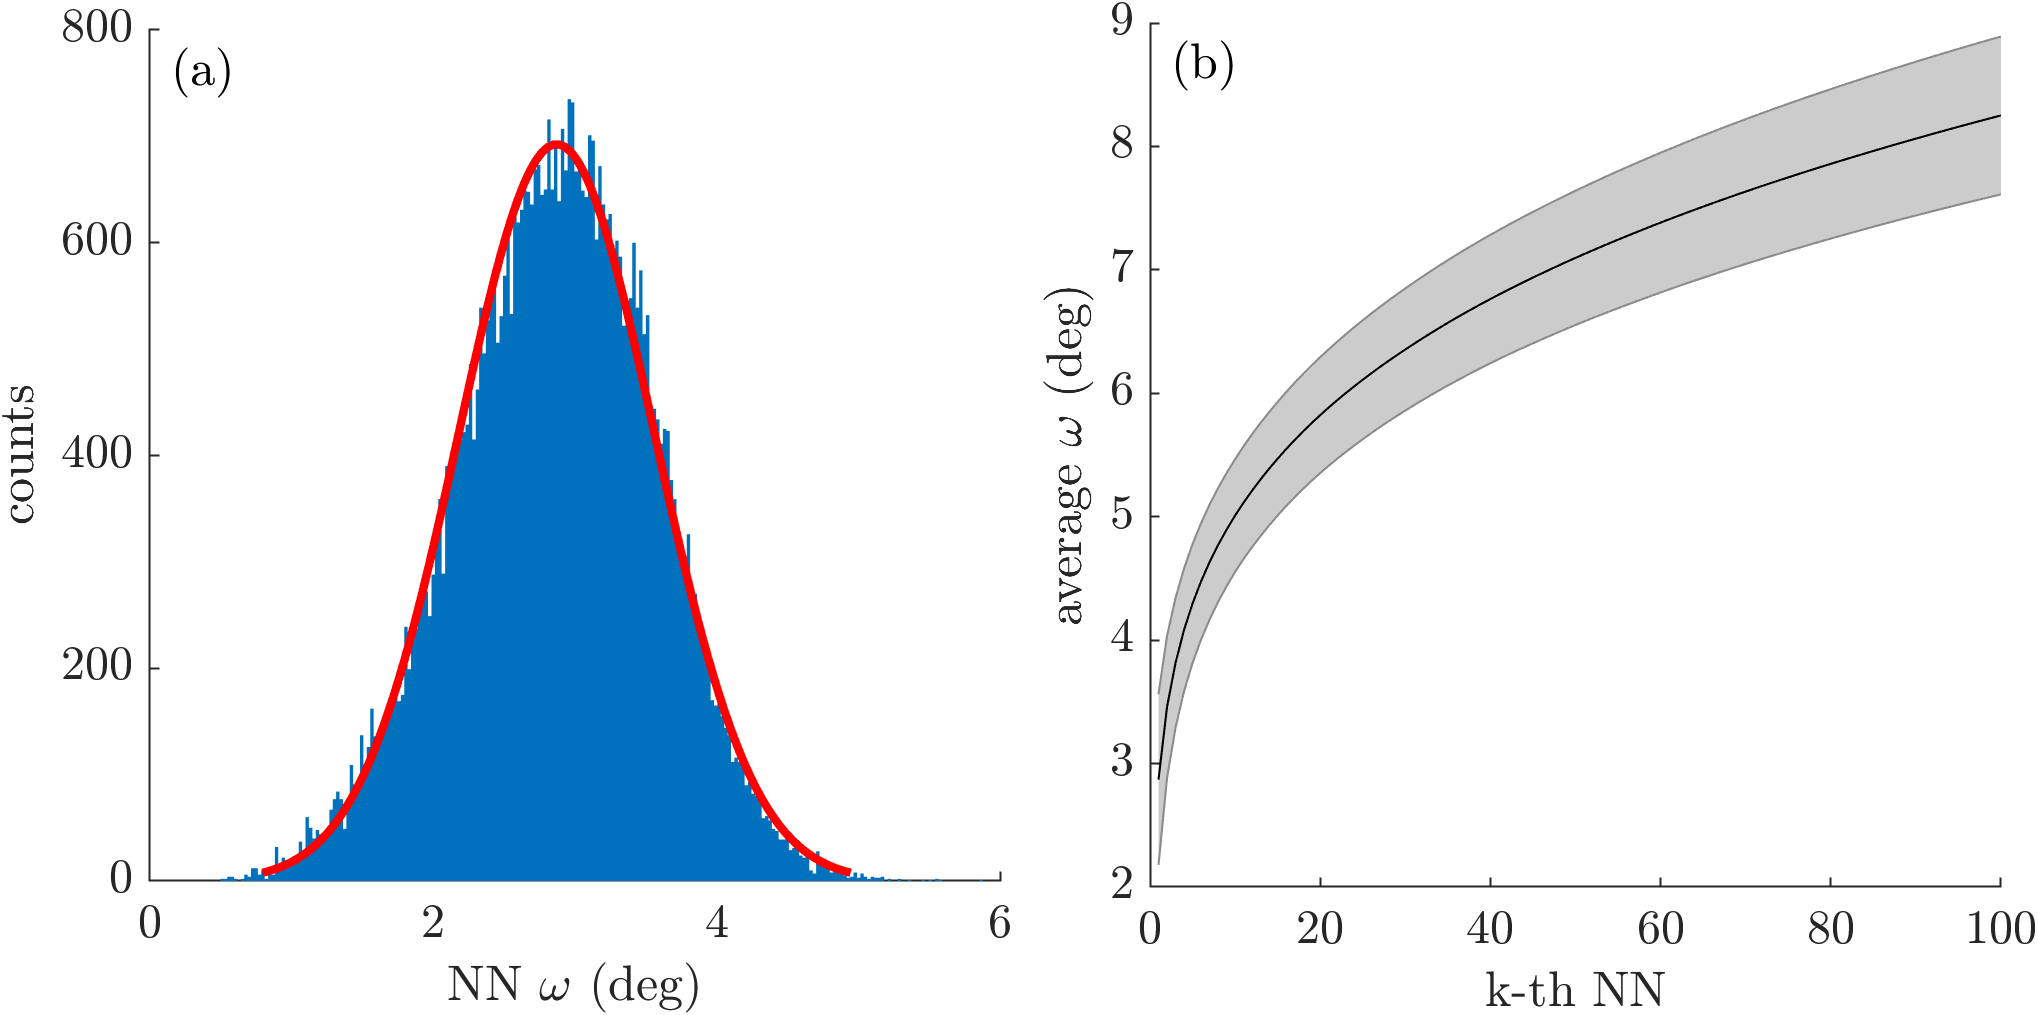
\includegraphics[scale=1]{nnhist-knn-50000.png}
\caption{Histogram of \gls{nn} octonion distances ($\omega$) in a \gls{vfzo} set of \num{50000} points. The mean and standard deviation are \SI{2.87}{\degree} and \SI{0.7}{\degree}, respectively.} %Histogram of \acrlong{nn} octonion distances ($\omega$) for the vertices of the vfz triangulation used for testing. The mean and standard deviation are \SI{2.87}{\degree} and \SI{0.7}{\degree}, respectively.
\label{fig:nnhist-knn-50000}
\end{figure}

\subsection{Interpolation Accuracy}
\label{sec:results:accuracy}

\Cref{fig:brkparity50000} provides hexagonally binned parity plots \cite{beanHexscatter2020} for each of the four interpolation methods.
\begin{figure}
    \centering
    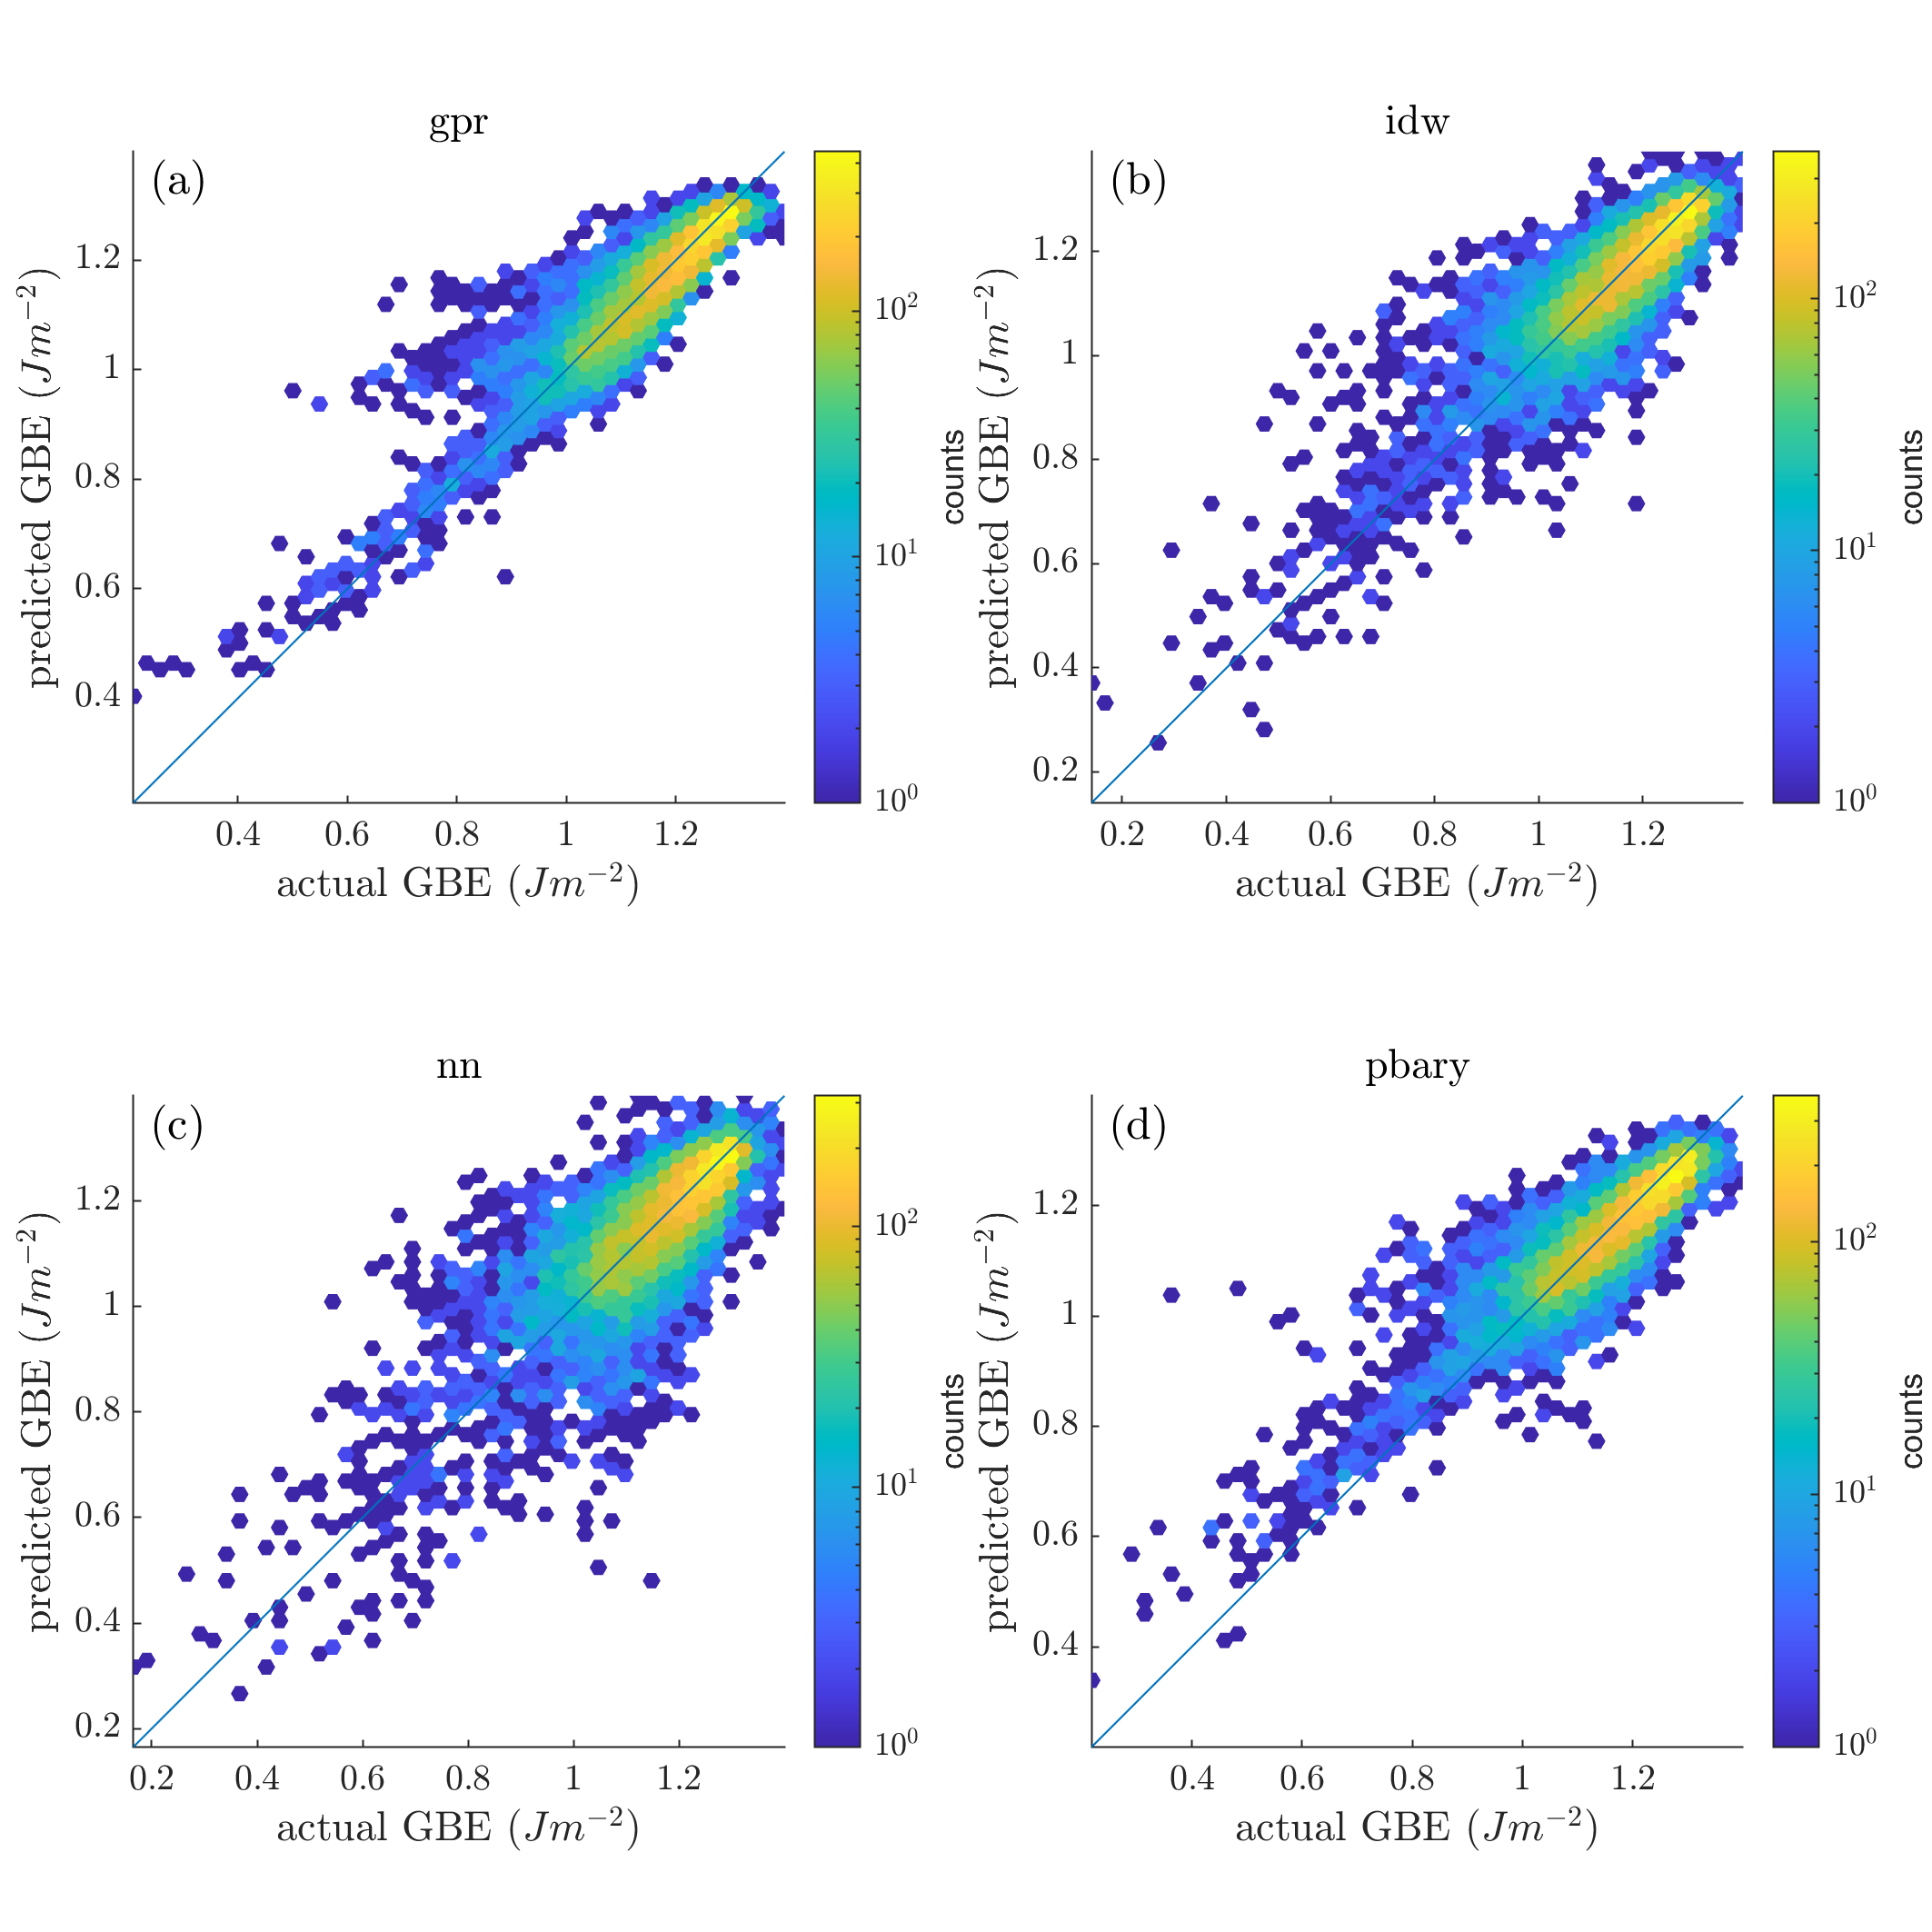
\includegraphics[scale=1]{brkparity50000.png}
    \caption{Hexagonally binned parity plots for \num{50000} mesh and \num{10000} prediction octonions formed via pairs of a random cubochorically sampled quaternion and a spherically sampled random boundary plane normal. Interpolation via (a) \acrlong{gpr}, (b) \acrlong{idw}, (c) \acrlong{nn}, and (d) barycentric coordinates.  \acrlong{brk} \acrlong{gbe} function for \gls{fcc} Ni was used as the test function.}
    \label{fig:brkparity50000}
\end{figure}

All of the methods permit successful interpolation, and the highest density region in all cases falls squarely on the parity line. The \Gls{gpr} and barycentric results show a slight asymmetry such that low energy values are overpredicted more often than they are underpredicted. The width of the point clouds provides a qualitative indication of the dispersion in the prediction errors. Quantitative measures of the overall accuracy are presented for \gls{rmse} (\cref{tab:rmse-error-comparison}) and \gls{mae} (\cref{tab:mae-error-comparison}) along with results of prior work where available.

\begin{table}
\caption{Comparison of average interpolation error for each interpolation method in the present work, using \num{50000} points in the definition of the \gls{vfz}. Comparison to the work of other authors is also included. A constant model (Cst, Avg \gls{rmse}), whose value was chosen to be the mean of the input \gls{gbe} was used as a control, except in the case of \gls{lobpcg} which used the mean of the true \gls{gbe} values instead. The last two columns, \gls{rmse} $\downarrow$ (\SI{}{\J\per\square\meter} and \gls{rmse}   $\downarrow$ (\%)), represent the reduction in \gls{rmse} in units of \SI{}{\J\per\square\meter} and \% relative to the control model, respectively.}
\centering
\begin{tabular}{lccccc}
\toprule
Method &
  \thead{\# \glspl{gb}} &
  \thead{\gls{rmse} \\   (\SI{}{\J\per\square\meter})} &
  \thead{Cst, Avg \gls{rmse} \\   (\SI{}{\J\per\square\meter})} &
  \thead{\gls{rmse} $\downarrow$ \\   (\SI{}{\J\per\square\meter})} &
  \thead{\gls{rmse}   $\downarrow$ \\ (\%)} \\ \midrule
\Gls{gpr}                                                     & \num{50000}  & \num{0.0541} & \num{0.1296} & \num{0.0755} & \num{58.3} \\
Barycentric                                                   & \num{50000}  & \num{0.0607} & \num{0.1296} & \num{0.0689} & \num{53.2} \\
\gls{idw}                                                     & \num{50000}  & \num{0.068}  & \num{0.1296} & \num{0.0616} & \num{47.5} \\
\gls{nn}                                                      & \num{50000}  & \num{0.0821} & \num{0.1296} & \num{0.0475} & \num{36.7} \\
\gls{lobpcg}   \cite{shenDeterminingGrainBoundary2019}        & \num{180000} & \num{0.0092} & \num{0.0976} & \num{0.0884} & \num{90.6} \\
\gls{ann}   \cite{echeverrirestrepoUsingArtificialNeural2014} & \num{17176}  & \NA          & \num{0.0854} & \NA          & \NA        \\
\gls{lkr}   \cite{chesserLearningGrainBoundary2020}           & \num{388}    & \num{0.0977} & \num{0.2243} & \num{0.1266} & \num{56.4} \\ \bottomrule
\end{tabular}
\label{tab:rmse-error-comparison}
\end{table}

% \begin{table}
% \caption{Comparison of average interpolation error for each interpolation method in the present work, using \num{50000} points in the definition of the vfz. Comparison to the work of other authors is also included. A constant model, whose value was chosen to be the mean of \texttt{f\_v}, was used as a control.}
% \centering
% \begin{tabular}{lccc}
% \toprule
% Method                                                & \multicolumn{1}{l}{\# \glspl{gb}} & \multicolumn{1}{l}{Cst, Avg \gls{mae} (\SI{}{\J\per\square\meter})} & \multicolumn{1}{l}{\gls{mae} (\SI{}{\J\per\square\meter})} \\ \midrule
% \Gls{gpr}                                             & \num{50000}                       & \num{0.0964}                                                        & \num{0.0372}                                               \\
% Barycentric                                           & \num{50000}                       & \num{0.0964}                                                        & \num{0.0418}                                               \\
% \gls{idw}                                             & \num{50000}                       & \num{0.0964}                                                        & \num{0.0470}                                               \\
% \gls{nn}                                              & \num{50000}                       & \num{0.0964}                                                        & \num{0.0573}                                               \\
% LOBPCG \cite{shenDeterminingGrainBoundary2019}        & \num{180000}                      & \num{0.0466}                                                        & N/A                                                        \\
% ANN \cite{echeverrirestrepoUsingArtificialNeural2014} & \num{17176}                       & \num{0.0617}                                                        & \num{0.0486}--\num{0.085}                                  \\
% LKR \cite{chesserLearningGrainBoundary2020}           & \num{388}                         & \num{0.1752}                                                        & \num{0.0977}                                               \\ \bottomrule
% \end{tabular}
% \label{tab:mae-error-comparison}
% \end{table}

\begin{table}
\caption{Comparison of average interpolation error for each interpolation method in the present work, using \num{50000} points in the definition of the \gls{vfz}. Comparison to the work of other authors is also included. A constant model (Cst, Avg \gls{mae}), whose value was chosen to be the mean of the input \gls{gbe} was used as a control. The last two columns, \gls{mae} $\downarrow$ (\SI{}{\J\per\square\meter} and \gls{mae}   $\downarrow$ (\%)), represent the reduction in \gls{mae} in absolute units of \SI{}{\J\per\square\meter} and \% relative to the control model, respectively.}
\centering
\begin{tabular}{lccccc}
\toprule
Method &
  \# \glspl{gb} &
  \thead{\gls{mae} \\   (\SI{}{\J\per\square\meter})} &
  \thead{Cst, Avg \gls{mae} \\   (\SI{}{\J\per\square\meter})} &
  \thead{\gls{mae} $\downarrow$ \\   (\SI{}{\J\per\square\meter})} &
  \thead{\gls{mae}   $\downarrow$ \\ (\%)} \\ \midrule
\Gls{gpr}                                                     & \num{50000}  & \num{0.0372} & \num{0.0964} & \num{0.0592} & \num{61.4} \\
Barycentric                                                   & \num{50000}  & \num{0.0418} & \num{0.0964} & \num{0.0546} & \num{56.6} \\
\gls{idw}                                                     & \num{50000}  & \num{0.047}  & \num{0.0964} & \num{0.0494} & \num{51.2} \\
\gls{nn}                                                      & \num{50000}  & \num{0.0573} & \num{0.0964} & \num{0.0391} & \num{40.6} \\
\gls{lobpcg}   \cite{shenDeterminingGrainBoundary2019}        & \num{180000} & \NA          & \num{0.0466} & \NA          & \NA        \\
\gls{ann}   \cite{echeverrirestrepoUsingArtificialNeural2014} & \num{17176}  & \num{0.0486} & \num{0.0617} & \num{0.0131} & \num{21.2} \\
\gls{lkr}   \cite{chesserLearningGrainBoundary2020}           & \num{388}    & \num{0.0977} & \num{0.1752} & \num{0.0775} & \num{44.2} \\ \bottomrule
\end{tabular}
\label{tab:mae-error-comparison}
\end{table}

% \begin{table}
% \caption{Comparison of average runtime for each interpolation method in the present work, using \num{50000} points in the definition of the \gls{vfz}. Comparison to the work of other authors is also included. A constant model, whose value was chosen to be the mean of \texttt{f\_v}, was used as a control.}
% \centering
% \begin{tabular}{lccc}
% \toprule
% Method & \# \glspl{gb} & Runtime (\SI{}{\second}) \\
% \midrule
% \Gls{gpr} & x & x \\
% Barycentric & x & x \\
% \gls{idw} & x & x \\
% \gls{nn} & x & x \\
% Constant & 0.13 & 0.097 \\
% LOBPCG \cite{shenDeterminingGrainBoundary2019} & 0.01--0.03 & --- \\
% ANN \cite{echeverrirestrepoUsingArtificialNeural2014} & --- & 0.05--0.09 \\
% LKR \cite{chesserLearningGrainBoundary2020} & 0.0977 & --- \\
% \bottomrule
% \end{tabular}
% \label{tab:runtime-comparison}
% \end{table}

To aid in objective interpretation of the error metrics, comparison is made to a constant valued control model, whose value is chosen to be the average of \texttt{f\_v} (approximately \SI{1.16}{\J\per\square\meter} in the limit of $nmeshpts \rightarrow \infty$) resulting in \gls{rmse} and \gls{mae} values of approximately \num{0.130} and \SI{0.097}{\J\per\square\meter}. Because the true models differed for other articles, equivalent errors obtained by a constant valued control model (mean of input \gls{gbe} values\footnote{Because \cite{shenDeterminingGrainBoundary2019} uses polycrystal rather than bicrystal data, for which there is no direct measure of the \gls{gbe}, the mean of the true \glspl{gbe} is used instead.}) were also included for prior work in \cref{tab:rmse-error-comparison} and \cref{tab:mae-error-comparison}. These metrics give a sense of the complexity and variability of the true function being inferred and allow for a more objective comparison between differing works.

Of the four interpolation methods from this work, \Gls{gpr} has the lowest error, both in terms of \gls{rmse} and \gls{mae}, while \gls{nn} has the highest error. % ... Add comments comparing the performance of the methods in \cref{tab:error-comparison} to the constant value and the literature methods. This is where we highlight that your method outperforms prior work.

The accuracy of the predictions made using the \gls{vfz} methods depends on the resolution of the \gls{vfz} triangulation. \Cref{fig:brkerror} compares the prediction accuracy for each of the 4 methods to the constant valued control model, as a function of the number of mesh vertices (\texttt{nmeshpts}). As expected, higher density \gls{vfz} point sets result in lower error and diminishing returns (\cref{fig:brkerror}). Moreover, the standard deviations produced via multiple runs are tightly constrained and generally shrink as the mesh size increases. 

\Gls{gpr} consistently gives lower error than the other three interpolation methods. It is interesting to see that despite qualitative differences in the parity plots for barycentric and \gls{idw} interpolation, these two methods produce similar \gls{rmse} and \gls{mae} values. \Gls{nn} interpolation produces the worst error of the four methods, but is better than the constant valued control model above several hundred input points. 

Both \gls{gpr} and \gls{idw} seem to reach a plateau near 20,000 input points. It is worthwhile to note that both of these methods are kernel-based in that a model parameter controls the size of the region that can influence the interpolation results. In the \gls{gpr} case, this is automatically calculated via an internal fitting routine of \texttt{fitrgp()}. \gls{nn} mesh distance distributions (\cref{fig:nnhist-knn-50000}) can lead to insight about correlation lengths in a given mesh. In the \gls{idw} case, the radius of influence is set to $r=\sqrt{2} \mu$, where $\mu$ is the mean \gls{nn} mesh distance. It is likely that better tuning of the kernel parameters in these two methods could further decrease the obtained errors. By contrast, barycentric interpolation automatically adjusts its effective region of influence because the size of the simplices in the mesh decreases as the number of vertices increases. More uniformly distributed meshes (such as obtained via constrained optimization \cite{dolanBenchmarkingOptimizationSoftware2004,ConstrainedElectrostaticNonlinear2020}) will likely result in more uniform, decreased interpolation error, especially for a simplex-based approach which is prone to high-aspect ratio facets. % However, this may be computationally infeasible for large mesh sizes.

% While not implemented in this work, it is expected that an \gls{ann} such as in \cite{echeverrirestrepoUsingArtificialNeural2014} could lead to even lower interpolation error than \gls{gpr} for large mesh sizes. % (e.g. https://www.mathworks.com/help/deeplearning/ref/narxnet.html, https://www.mathworks.com/help/deeplearning/function-approximation-and-nonlinear-regression.html)

\begin{figure}
    \centering
    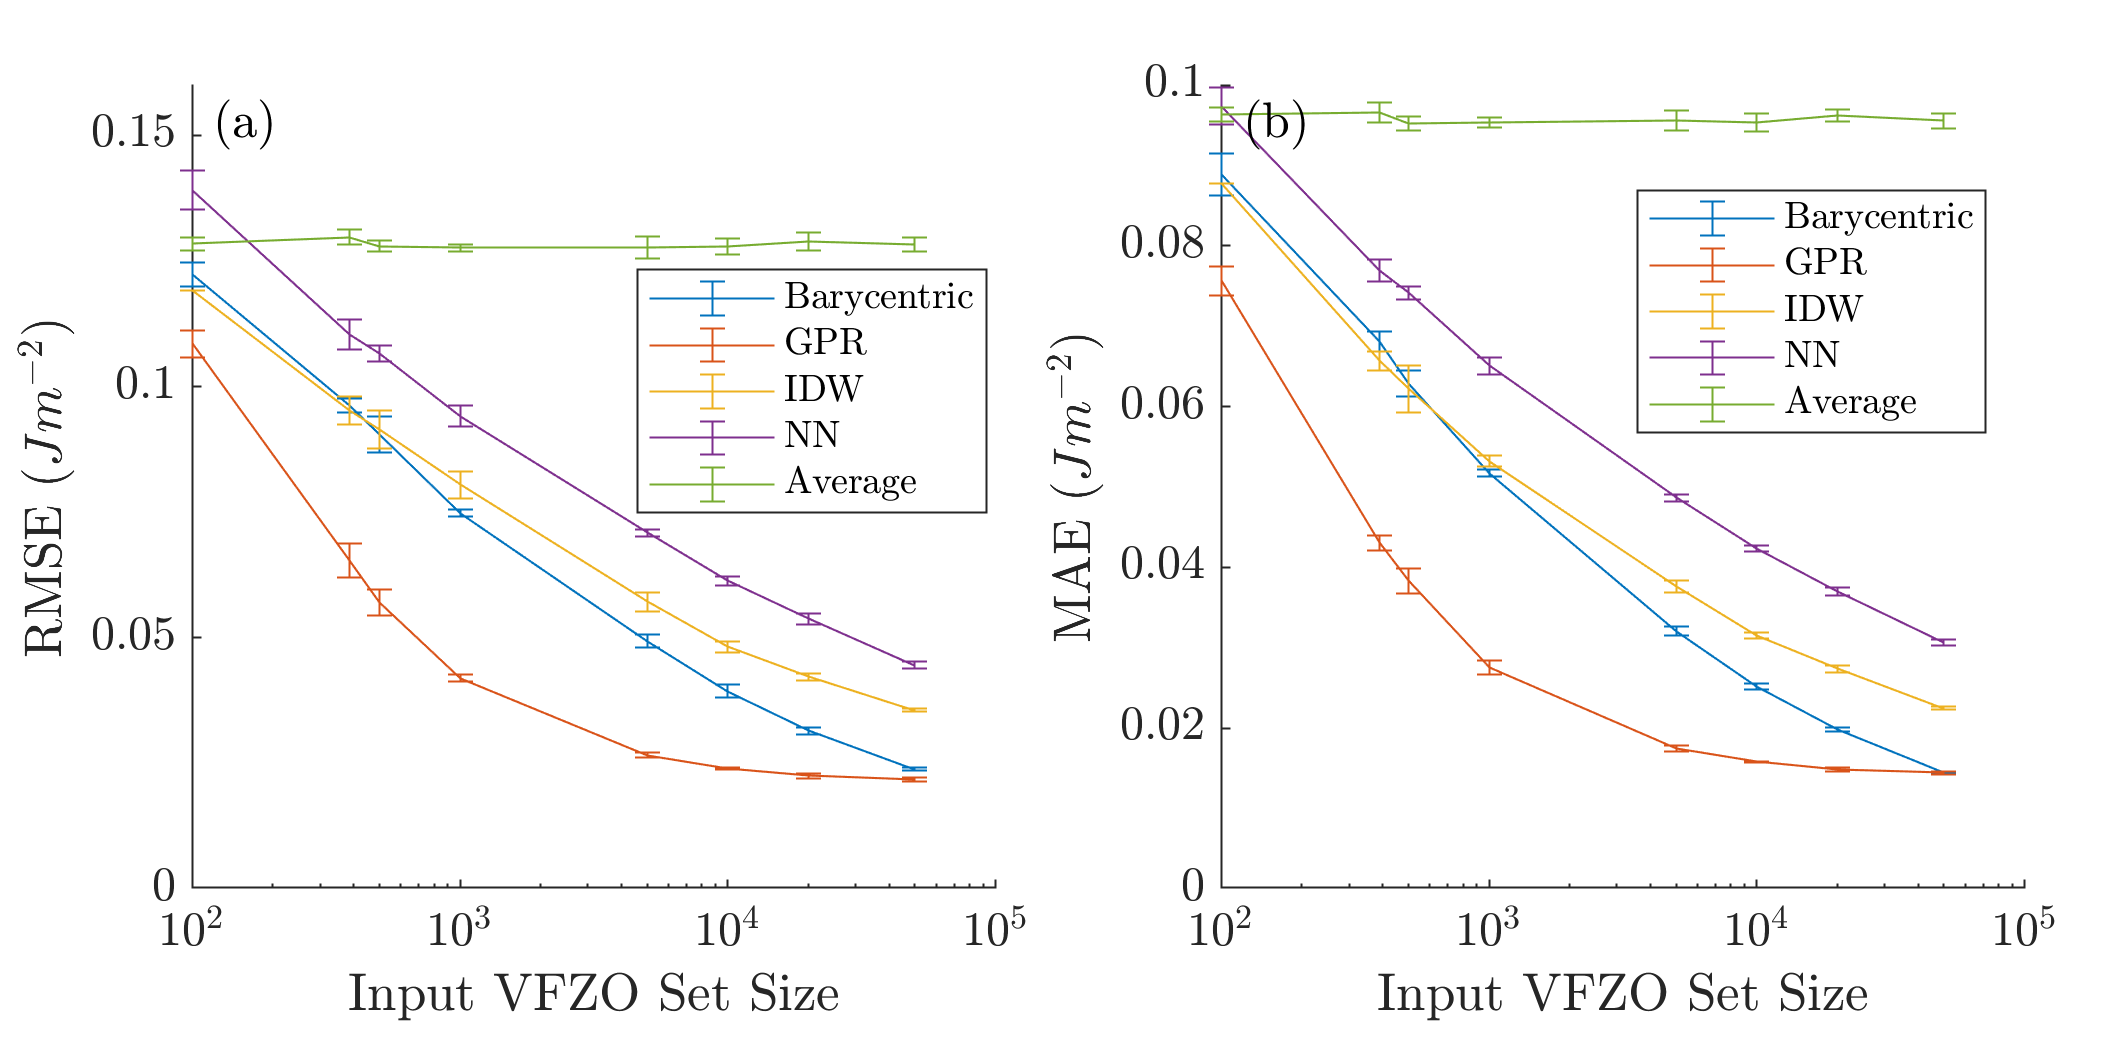
\includegraphics[scale=1]{brkerror.png}
    \caption{Average \gls{rmse} and average \gls{mae} vs. number of input points for planar barycentric (\texttt{pbary}, blue), \gls{gpr} (\texttt{gpr}, orange), \gls{idw} (\texttt{idw}, yellow), and \texttt{nn} (\texttt{nn}, purple) interpolation for approximately 10 random runs with different mesh and prediction points. Standard deviations of approximately 10 runs are also included. Compare with approximately \SI{0.13}{\J\per\square\meter} and \SI{0.95}{\J\per\square\meter} \gls{rmse} and \gls{mae}, respectively, for a constant model using the average of the mesh properties (approximately \SI{1.16}{\J\per\square\meter}).}
    %Average \acrlong{rmse} and average \acrlong{mae} vs. number of mesh points for planar barycentric (\texttt{pbary}, blue), \acrlong{gpr} (\texttt{gpr}, orange), \acrlong{idw} (\texttt{idw}, yellow), and \texttt{nn} (\texttt{nn}, purple) interpolation for approximately 10 random runs with different mesh and prediction points. Standard deviations of approximately 10 runs are also included. Compare with approximately \SI{0.13}{\J\per\square\meter} and \SI{0.95}{\J\per\square\meter} \acrshort{rmse} and \acrshort{mae}, respectively, for a constant model using the average of the mesh properties (approximately \SI{1.16}{\J\per\square\meter}).
    \label{fig:brkerror}
\end{figure}

\subsection{Interpolation Efficiency}
\label{sec:results:efficiency}

% general overview statement about the interpolation time and memory requirements

\Gls{gpr} is fast and has lower error compared to barycentric interpolation; however, the entire process has to be rerun (in current implementation) if the responses or the predictors change. On the other hand, barycentric interpolation is fast once the triangulation and intersections are computed. In other words, it is fast if only responses (i.e. \glspl{gbe}) change, but slow if the input points or predictors (i.e. \glspl{gb}) change.

Computational runtimes of the various interpolation methods are also shown (\cref{fig:runtime}). Barycentric interpolation takes the longest, which is compounded by the fact that it is the only parallelized method by default (not accounted for in \cref{fig:runtime}). In other words, since 12 cores were used to obtain these runtime results, the total runtime across all cores is much higher compared with the other methods; however, it is possible that other methods used multi-threading via built-in vectorized functions. The long computation times result primarily from the large number of facets present in a high-dimensional mesh triangulation and the interconnectedness of facets with respect to each other.

\Gls{gpr} is the second-longest in terms of of runtime, but produces better error than any of the other three methods. \Gls{nn} and \gls{idw} interpolation have vectorized implementations and are much simpler than the barycentric and \gls{gpr} methods. Consistent with expectations, \gls{nn} and \gls{idw} exhibit almost negligible runtimes; however, this is at the expense of error trade-offs discussed earlier (\cref{sec:results:accuracy}). It should also be noted that barycentric interpolation and \gls{gpr} have much higher memory requirements than \gls{nn} and \gls{idw} due to the need to store large matrices (unless \texttt{fitrgp PredictMethod = 'fic'}).

Because the default implementation of \gls{idw} uses a radius cut-off, the distance and weight matrices can be stored as sparse objects, dramatically reducing both the storage requirements and computational complexity of this method. We expect that a \gls{knn} approach would produce similar results both in terms of runtime and error when a relatively uniform sampling of \gls{gbc} is obtained.

\begin{figure}
    \centering
    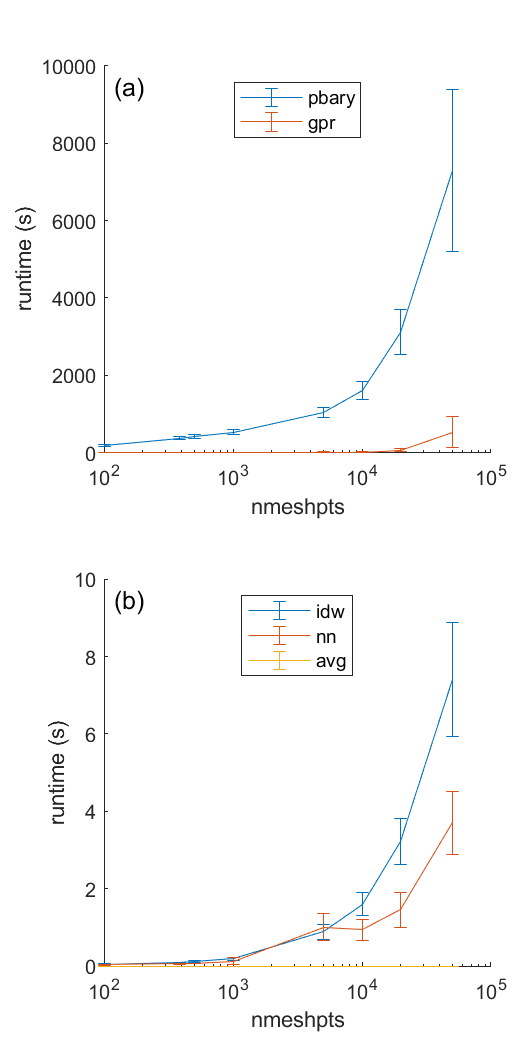
\includegraphics[scale=1]{runtime.png}
    \caption{
    Average runtime (s) and standard deviation (approximately 10 runs) vs. number of input points for barycentric (a, blue) and \acrlong{gpr} (\acrshort{gpr}) (a, orange), \acrlong{idw} (\acrshort{idw}) (b, blue), \acrlong{nn} (\acrshort{nn}) (b, orange) interpolation using 12 cores compared against runtime (s) for an average model (b, yellow). Because \acrshort{gpr}, \acrshort{idw}, and \acrshort{nn} method defaults do not use parfor loops but may have internal multi-core vectorization, it is unclear to what extent the number of cores affects the runtime of methods other than barycentric interpolation. \Acrlong{gb} symmetrization runtime was not included; however, symmetrization takes approximately one minute on 6 cores (Intel i7-10750H, 2.6 GHz) and is a common step in every interpolation method (i.e. it is fundamental to the \acrlong{vfzo} framework).
    %Runtime (s) vs. number of mesh points for barycentric (blue), \acrlong{gpr} (\acrshort{gpr}) (orange), \acrlong{idw} (\acrshort{idw}) (yellow), and \acrlong{nn} (\acrshort{nn}) (purple) interpolation using 12 cores. Because \acrshort{gpr}, \acrshort{idw}, and \acrshort{nn} method defaults do not use parfor loops but may have internal multi-core vectorization, it is unclear to what extent the number of cores affects the runtime of methods other than barycentric interpolation. \Acrlong{gb} symmetrization runtime was not included; however, symmetrization takes approximately one minute on 6 cores (Intel i7-10750H, 2.6 GHz) and is a common step in every interpolation method (i.e. it is fundamental to the \acrlong{vfzo} framework).
    }
    \label{fig:runtime}
\end{figure}

\section{Conclusion} \label{sec:conclusion}

A high fidelity \gls{vfzo} framework for interpolation of \gls{gb} properties is presented and four interpolation schemes built on the \gls{vfzo} framework are described and tested. This framework enables faster computation of pairwise distance matrices and produces lower error than previous methods.
%similar error to a machine learning approach that does not consider symmetrically equivalent \glspl{gb} \cite{echeverrirestrepoUsingArtificialNeural2014}.
%Barycentric, \gls{gpr}, and \gls{idw} always yield lower error than pure \gls{nn} interpolation (\cref{fig:brkparity50000}), especially for large mesh sizes.
The approach is general to any crystal system (which can be selected by the parameter \texttt{pgnum}). \Gls{gpr} is demonstrated to offer a competitive advantage in computation time and error relative to barycentric, \gls{idw}, and \gls{nn} interpolation, which were also considered in this work. \Gls{gpr} is the the generally recommended interpolation method for the \gls{vfzo} framework; however, the other methods can meet niche needs. An easy-to-use, versatile interpolation function is provided (\url{github.com/sgbaird-5dof/interp}, \cite{bairdFiveDegreeofFreedom5DOF2020}). We anticipate that the \gls{vfzo} framework and corresponding implementation will enable many advances in the field of \gls{gb} structure-property models and surrogates.
    
% \subsection{Future Work} \label{sec:conclusions:future}

% \subsubsection{\glsentrytitlecase{fz}{long}}
% It is unclear how difficult it would be to define \gls{fz} borders with high-symmetry GBs on the perimeter, and it is possible that the borders would exhibit curvature. Ideally, a convex hull of the points that define such a border would also define a \gls{fz}; however, if the borders have curvature, this is not guaranteed. An additional advantage of the \gls{vfzo} framework is the possibility of defining discontinuous or "sharp" features within a closed-mesh using existing methods such as in \cite{tianNonUniformSubdivisionSurfaces2020}. Because high-symmetry \glspl{gb} can be sampled via knowledge of misorientation and \gls{bp} \glspl{fz} and may even have generalized, analytical representations in octonion space, such an approach has great potential to increase interpolation accuracy of methods built on the \gls{vfzo} framework (especially near high-symmetry grain boundaries). Exaggerated errors may also arise for \glspl{gb} near the low-symmetry exterior of the mesh. In lieu of defining every \gls{seo} of every mesh point, ensemble methods can be employed to combat these interpolation inaccuracies. We think it is reasonable to expect that a low number of components in an ensemble (e.g. 8) could negate exaggerations in errors near mesh-exteriors. For example, instead of using a single reference octonion, a low number of reference octonions with maximized pairwise-distances \cite{dolanBenchmarkingOptimizationSoftware2004,ConstrainedElectrostaticNonlinear2020} with respect to each other can define multiple meshes and ensure that every \gls{gb} is situated reasonably far from the mesh exterior for at least one mesh in the ensemble. It may be necessary to first explore the source of error bias (Section \cref{results:general:bias}) to verify that higher error preferentially occurs near the \gls{fz} exterior.

% \subsubsection{Other Interpolation Methods}
% Including an ensemble approach described above, other options for continuing this work involve extending linear interpolation methods to hyperspherical spline interpolation \cite{taijeronSplineInterpolationSmoothing1994}. Unfortunately, built-in MATLAB spline interpolations require gridded (as opposed to scattered) data in high dimensions (four or higher in \textit{spapi} and \textit{interpn}), so an alternative implementation is likely required. A gridded mesh could be defined; however, due to the curse-of-dimensionality and the fact that \glspl{gbo} are on the surface of a hypersphere, an unreasonably large number of points compared to the methods described here and/or an rigid \gls{svd} transformation to 6D Cartesian (neither distance- nor angle-preserving) would likely be required. Generalized barycentric coordinates \cite{floaterGeneralizedBarycentricCoordinates2015,meyerGeneralizedBarycentricCoordinates2002,langerSphericalBarycentricCoordinates2006} are another implementation option which could potentially speed up and improve error in barycentric interpolation time since the number of vertices per facet can increase. It is also likely that for large mesh sizes (e.g. \num{10000}+ mesh points), an \gls{ann} approach \cite{echeverrirestrepoUsingArtificialNeural2014} could also decrease interpolation error while maintaining low computation times. Further optimization of hyperparameters used in this work, such as for noise standard deviation and smoothness length in \gls{gpr} may lead to lower model error.

% \subsubsection{Other \glsentrytitlecase{gb}{long} Distance Metrics}
% Barycentric interpolation using other \gls{gb} distance metrics \cite{morawiecDistancesGrainInterfaces2019} could also be performed by recomputing barycentric coordinates in a \gls{vfzo} triangulation, supplying octonion facet vertices to a simplex reconstruction using only edge lengths computed by the alternative distance metric \cite{connorHighdimensionalSimplexesSupermetric2017}, or by computing a manifold from only a pairwise distance matrix \cite{boissonnatOnlyDistancesAre2017}.

% \subsubsection{Applications}
% We think it is straightforward to apply these methods to full or restricted regions of \gls{5dof} space for \gls{gb} models and surrogates. In addition to interpolations involving \gls{gbe}, \gls{gbcd} (i.e. similar to fitting a curve to a histogram) and other \gls{gb} properties such as diffusivity and mobility could also be interpolated. Finally, linking this interpolation scheme with polycrystal data such as 3D microstructural \gls{tj} datasets (e.g. Ni \cite{liRelativeGrainBoundary2009}) via \textit{TJ2GBE} \cite{shenDeterminingGrainBoundary2019} or similar approaches geared towards large datasets is especially promising.


% \section{Supplemental}
% \begin{enumerate}
%     \item conversion from octonion to \gls{5dof}
%     \item high-aspect ratio facets
%     \item facet subdivision
%     \item spherical vs. planar barycentric interpolation
%     \item tolerances of interpolation and intersecting facets
%     \item non-intersection percentage vs. number of mesh points
%     \item "excess" arc length in pairwise distance matrices
%     \begin{enumerate}
%         \item gradient optimization and global optimization of U(1) twist symmetry with marginal improvement
%     \end{enumerate}
%     \item identification and subdivision of hull exterior
%     \item distribution of data in \gls{mfz} and \gls{bp} spaces
%     \item comments on \gls{gpr} hyperparameters
% \end{enumerate}

\appendix
\label{sec:app}
\section{Detailed Barycentric Interpolation Methods}
\setcounter{figure}{0}
\subsection{Triangulating a \glsentrytitlecase{vfz}{long} Mesh}
\label{app:bary-tri}

% Briefly (but clearly and explicitly) explain the steps of generating the cubochorically sampled GBs, converting them to octonions and then mapping all of them into the vfz. Then explain how you do the triangulation. This will require a few figures to show the process in 3D (i.e. generating a triangulation of a point cloud on a region of the surface of the 2-sphere).

% After random \glspl{vfzo} are obtained (\cref{sec:methods:rand}), % ...

In order to reduce the computational complexity of triangulating a high-dimensional mesh \cite{barberQuickhullAlgorithmConvex1996}, some simplifications are made. The degenerate dimension obtained from analytically minimizing $U(1)$ symmetry \cite{francisGeodesicOctonionMetric2019} is first removed via a rigid (i.e. distance- and angle-preserving) \gls{svd} transformation,
%to enable use of MATLAB's quickhull \cite{barberQuickhullAlgorithmConvex1996} implementations such as \texttt{delaunayn} and \texttt{convhulln}. Removal of the degenerate dimension is done via a rigid \gls{svd} transformation,
analogous to a Cartesian rotation and translation
%Thus, a set of octonions originally represented by 8D Cartesian coordinates are collapsed to a 7D Cartesian representation while preserving both distances and angles among the points
As a 3D Cartesian to 2D Cartesian analogue of this 8D Cartesian to 7D Cartesian transformation, we take a set . Next, this 7D Cartesian representation is projected onto a hyperplane tangent to the mean of the input points\footnote{This is \textit{not} a rigid transformation; however, it is sufficiently close to produce a high-quality triangulation in a \gls{vfz}.} (\cref{fig:bary-delaunay}b). The 7D Cartesian \glspl{gbo} undergo another rigid \gls{svd} transformation to 6D Cartesian (see 3D to 2D analogue in \cref{fig:bary-delaunay}c) for which a triangulation is computed via the quickhull algorithm \cite{barberQuickhullAlgorithmConvex1996} (see MATLAB function \texttt{delaunayn}).

\begin{figure}
    \centering
    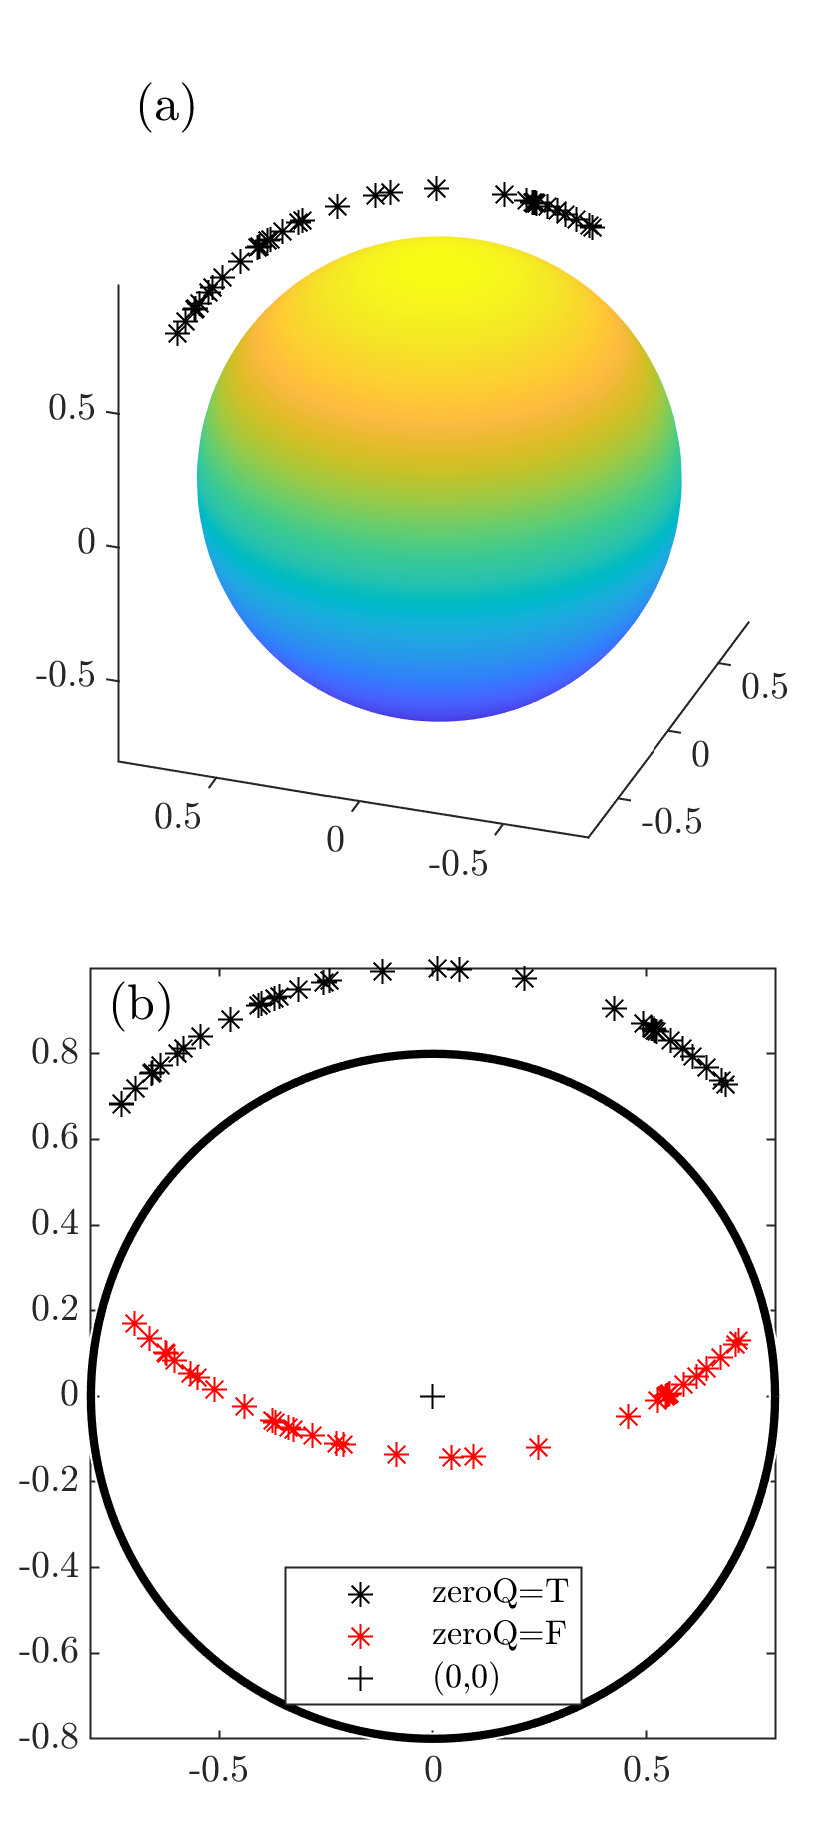
\includegraphics[scale=1]{bary-remove-deg.png}
    \caption{3D Cartesian to 2D Cartesian analogue of 8D Cartesian to 7D Cartesian degeneracy removal used in barycentric interpolation approach. Starting spherical arc points on surface of 2-sphere (a) and degenerate dimension removed via \acrlong{svd} transformation to 2D Cartesian (b) with either the origin (black plus) preserved (black asterisks, \texttt{zeroQ=T}) or ignored (red asterisks, \texttt{zeroQ=F}). The sphere (a) and circle (b) each have a radius of 0.8 and are used as a visualization aid only.}
    \label{fig:bary-remove-deg}
\end{figure}

Using a separate rigid \gls{svd} transformation from the triangulation, the original mesh and prediction \glspl{gbo} are simultaneously transformed from 8D Cartesian to 7D Cartesian. Because our \gls{svd} approach is rigid, the triangulation is then superimposed onto the newly transformed input points resulting in a 7D Cartesian \gls{vfz}.

\begin{figure}
    \centering
    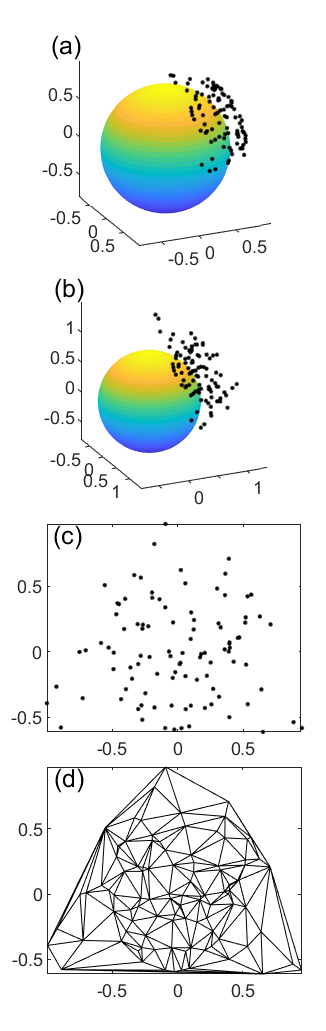
\includegraphics[scale=1]{bary-delaunay.png}
    \caption{3D Cartesian to 2D Cartesian analogue of 7D Cartesian to 6D Cartesian mesh triangulation used in barycentric interpolation approach. Input points linearly projected projected onto hyperplane tangent to mean of starting points (a), degenerate dimension removed via rigid \gls{svd} transformation to 2D Cartesian and Delaunay triangulation calculated (b), and Delaunay triangulation superimposed onto normalized input points. The spheres in (a) and (c) have a radius of 0.8 and is used for visualization only.}
    \label{fig:bary-delaunay}
\end{figure}

% In order to reduce the computationally complexity of computing barycentric coordinates in a high-dimensional space \cite{barberQuickhullAlgorithmConvex1996}, a single degenerate dimension (originally introduced by analytically minimizing $U(1)$ symmetry) is removed to enable use of MATLAB's quickhull \cite{barberQuickhullAlgorithmConvex1996} implementations such as \texttt{delaunayn} and \texttt{convhulln}. Removal of the degenerate dimension is done via a rigid \gls{svd} transformation, analogous to a Cartesian rotation and translation. Thus, a set of octonions originally represented by 8D Cartesian coordinates are collapsed to a 7D Cartesian representation while preserving both distances and angles among the points (see 3D to 2D analogue in \cref{fig:bary-remove-deg}). To further reduce the "curse of dimensionality" in computing the triangulation, a 7D Cartesian representation of the octonions constrained to lie on the surface of the 6-sphere are first projected onto a hyperplane tangent to the mean of the input points and then rotated/translated again via \gls{svd} to produce a 6D Cartesian representation (see 3D to 2D analogue in Figure \cref{fig:bary-delaunay}). This 6D representation is used to compute a triangulation via the built-in MATLAB routine \texttt{delaunayn} based on the quickhull algorithm \cite{barberQuickhullAlgorithmConvex1996}, giving facet vertices for the 7D Cartesian hypersphere.

\subsection{Intersections in a \glsentrytitlecase{vfz}{long} Mesh}
\label{app:bary-int}
An intersection is calculated by linearly projecting a prediction point onto the hyperplane defined by a mesh facet's vertices (\cref{fig:bary-interp}, computing barycentric coordinates within the facet, and testing for positivity \cite{langerSphericalBarycentricCoordinates2006}, and repeating this process until an intersection is found or a stop condition is reached (see \texttt{nnMax} below). If the prediction point is contained within the simplex, all of the barycentric weights (i.e. coordinates) are positive. If it outside the simplex, this constraint is violated. Due to the large number of facets per point of a high-dimensional
%simplex-based
triangulation
%and for computational speed,
prediction point intersections are calculated by considering facets connected to up to some number of mesh \glspl{nn} (\texttt{nnMax}) (in this work, \texttt{nnMax = 10}). For prediction points where no intersecting facet is found
%in these connected facets due to high-aspect ratio facets or prediction point falling outside the mesh within a given tolerance,
a \gls{nn} approach is used (\cref{sec:methods:interp:nn}), which represent average non-intersection rates of \SI{0.1207 \pm 1.02}{\percent} and \SI{0.68 \pm 0.11}{\percent} for input meshes of \num{388} and \num{50000}, respectively, for \num{10000} query points out of \num{10} trials.

\subsection{Interpolation via Barycentric Coordinates}
\label{app:bary-interp}

Once barycentric coordinates are computed for a prediction point within the input mesh, the interpolated value is found by taking the dot product of the barycentric coordinates and the properties of the corresponding vertices of the intersecting facet via
\begin{equation}
\label{eq:bary-interp}
v=\underset{i=1}{\overset{N}{\sum }}\lambda _i v_i
\end{equation}
where $\lambda$, $v$, $v_i$ and $N$, are the barycentric coordinates, interpolated property, property of the $i$th vertex of the intersecting facet, and number of vertices in a given facet ($N = 7$ for the degeneracy-free 6-sphere). A 2-sphere example is provided in \cref{fig:bary-interp}.

\begin{figure}
    \centering
    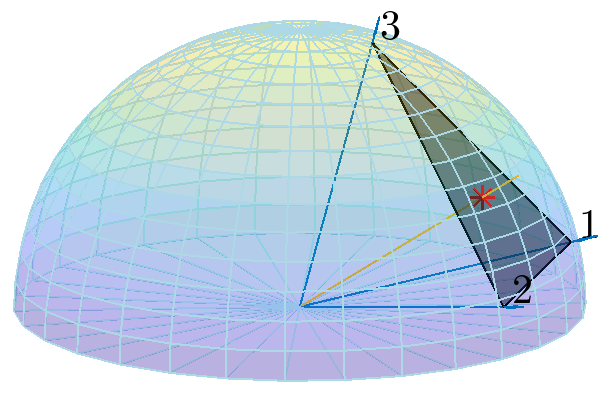
\includegraphics[scale=1]{bary-interp.png}
    \caption{A ray (red line) on the 2-sphere is linearly projected onto the hyperplane of a mesh facet (transparent black), shown as a red asterisk. The barycentric coordinates are computed as $\lambda_{i \in [1,3]} = \frac{1}{3}$. Because all barycentric coordinates are positive, it is determined that the projected point is an intersection with the mesh. Given vertex values of \num{8.183}, \num{3.446}, and \num{3.188} for vertices 1, 2, and 3, respectively, the interpolated value is calculated as \num{4.94} via \cref{eq:bary-interp}.}
    \label{fig:bary-interp}
\end{figure}

\newpage
\printglossaries
%need to manually clear cached files & logs in overleaf to get new abbreviations to appear

\newpage
\bibliographystyle{elsarticle-num-names}
\bibliography{5dof-gb-energy.bib}



\end{document}
